% Options for packages loaded elsewhere
\PassOptionsToPackage{unicode}{hyperref}
\PassOptionsToPackage{hyphens}{url}
\PassOptionsToPackage{dvipsnames,svgnames,x11names}{xcolor}
%
\documentclass[
  letterpaper,
  DIV=11,
  numbers=noendperiod]{scrreprt}

\usepackage{amsmath,amssymb}
\usepackage{iftex}
\ifPDFTeX
  \usepackage[T1]{fontenc}
  \usepackage[utf8]{inputenc}
  \usepackage{textcomp} % provide euro and other symbols
\else % if luatex or xetex
  \usepackage{unicode-math}
  \defaultfontfeatures{Scale=MatchLowercase}
  \defaultfontfeatures[\rmfamily]{Ligatures=TeX,Scale=1}
\fi
\usepackage{lmodern}
\ifPDFTeX\else  
    % xetex/luatex font selection
\fi
% Use upquote if available, for straight quotes in verbatim environments
\IfFileExists{upquote.sty}{\usepackage{upquote}}{}
\IfFileExists{microtype.sty}{% use microtype if available
  \usepackage[]{microtype}
  \UseMicrotypeSet[protrusion]{basicmath} % disable protrusion for tt fonts
}{}
\makeatletter
\@ifundefined{KOMAClassName}{% if non-KOMA class
  \IfFileExists{parskip.sty}{%
    \usepackage{parskip}
  }{% else
    \setlength{\parindent}{0pt}
    \setlength{\parskip}{6pt plus 2pt minus 1pt}}
}{% if KOMA class
  \KOMAoptions{parskip=half}}
\makeatother
\usepackage{xcolor}
\ifLuaTeX
  \usepackage{luacolor}
  \usepackage[soul]{lua-ul}
\else
  \usepackage{soul}
  
\fi
\setlength{\emergencystretch}{3em} % prevent overfull lines
\setcounter{secnumdepth}{5}
% Make \paragraph and \subparagraph free-standing
\makeatletter
\ifx\paragraph\undefined\else
  \let\oldparagraph\paragraph
  \renewcommand{\paragraph}{
    \@ifstar
      \xxxParagraphStar
      \xxxParagraphNoStar
  }
  \newcommand{\xxxParagraphStar}[1]{\oldparagraph*{#1}\mbox{}}
  \newcommand{\xxxParagraphNoStar}[1]{\oldparagraph{#1}\mbox{}}
\fi
\ifx\subparagraph\undefined\else
  \let\oldsubparagraph\subparagraph
  \renewcommand{\subparagraph}{
    \@ifstar
      \xxxSubParagraphStar
      \xxxSubParagraphNoStar
  }
  \newcommand{\xxxSubParagraphStar}[1]{\oldsubparagraph*{#1}\mbox{}}
  \newcommand{\xxxSubParagraphNoStar}[1]{\oldsubparagraph{#1}\mbox{}}
\fi
\makeatother


\providecommand{\tightlist}{%
  \setlength{\itemsep}{0pt}\setlength{\parskip}{0pt}}\usepackage{longtable,booktabs,array}
\usepackage{multirow}
\usepackage{calc} % for calculating minipage widths
% Correct order of tables after \paragraph or \subparagraph
\usepackage{etoolbox}
\makeatletter
\patchcmd\longtable{\par}{\if@noskipsec\mbox{}\fi\par}{}{}
\makeatother
% Allow footnotes in longtable head/foot
\IfFileExists{footnotehyper.sty}{\usepackage{footnotehyper}}{\usepackage{footnote}}
\makesavenoteenv{longtable}
\usepackage{graphicx}
\makeatletter
\newsavebox\pandoc@box
\newcommand*\pandocbounded[1]{% scales image to fit in text height/width
  \sbox\pandoc@box{#1}%
  \Gscale@div\@tempa{\textheight}{\dimexpr\ht\pandoc@box+\dp\pandoc@box\relax}%
  \Gscale@div\@tempb{\linewidth}{\wd\pandoc@box}%
  \ifdim\@tempb\p@<\@tempa\p@\let\@tempa\@tempb\fi% select the smaller of both
  \ifdim\@tempa\p@<\p@\scalebox{\@tempa}{\usebox\pandoc@box}%
  \else\usebox{\pandoc@box}%
  \fi%
}
% Set default figure placement to htbp
\def\fps@figure{htbp}
\makeatother
% definitions for citeproc citations
\NewDocumentCommand\citeproctext{}{}
\NewDocumentCommand\citeproc{mm}{%
  \begingroup\def\citeproctext{#2}\cite{#1}\endgroup}
\makeatletter
 % allow citations to break across lines
 \let\@cite@ofmt\@firstofone
 % avoid brackets around text for \cite:
 \def\@biblabel#1{}
 \def\@cite#1#2{{#1\if@tempswa , #2\fi}}
\makeatother
\newlength{\cslhangindent}
\setlength{\cslhangindent}{1.5em}
\newlength{\csllabelwidth}
\setlength{\csllabelwidth}{3em}
\newenvironment{CSLReferences}[2] % #1 hanging-indent, #2 entry-spacing
 {\begin{list}{}{%
  \setlength{\itemindent}{0pt}
  \setlength{\leftmargin}{0pt}
  \setlength{\parsep}{0pt}
  % turn on hanging indent if param 1 is 1
  \ifodd #1
   \setlength{\leftmargin}{\cslhangindent}
   \setlength{\itemindent}{-1\cslhangindent}
  \fi
  % set entry spacing
  \setlength{\itemsep}{#2\baselineskip}}}
 {\end{list}}
\usepackage{calc}
\newcommand{\CSLBlock}[1]{\hfill\break\parbox[t]{\linewidth}{\strut\ignorespaces#1\strut}}
\newcommand{\CSLLeftMargin}[1]{\parbox[t]{\csllabelwidth}{\strut#1\strut}}
\newcommand{\CSLRightInline}[1]{\parbox[t]{\linewidth - \csllabelwidth}{\strut#1\strut}}
\newcommand{\CSLIndent}[1]{\hspace{\cslhangindent}#1}

\KOMAoption{captions}{tableheading}
\makeatletter
\@ifpackageloaded{tcolorbox}{}{\usepackage[skins,breakable]{tcolorbox}}
\@ifpackageloaded{fontawesome5}{}{\usepackage{fontawesome5}}
\definecolor{quarto-callout-color}{HTML}{909090}
\definecolor{quarto-callout-note-color}{HTML}{0758E5}
\definecolor{quarto-callout-important-color}{HTML}{CC1914}
\definecolor{quarto-callout-warning-color}{HTML}{EB9113}
\definecolor{quarto-callout-tip-color}{HTML}{00A047}
\definecolor{quarto-callout-caution-color}{HTML}{FC5300}
\definecolor{quarto-callout-color-frame}{HTML}{acacac}
\definecolor{quarto-callout-note-color-frame}{HTML}{4582ec}
\definecolor{quarto-callout-important-color-frame}{HTML}{d9534f}
\definecolor{quarto-callout-warning-color-frame}{HTML}{f0ad4e}
\definecolor{quarto-callout-tip-color-frame}{HTML}{02b875}
\definecolor{quarto-callout-caution-color-frame}{HTML}{fd7e14}
\makeatother
\makeatletter
\@ifpackageloaded{bookmark}{}{\usepackage{bookmark}}
\makeatother
\makeatletter
\@ifpackageloaded{caption}{}{\usepackage{caption}}
\AtBeginDocument{%
\ifdefined\contentsname
  \renewcommand*\contentsname{Table of contents}
\else
  \newcommand\contentsname{Table of contents}
\fi
\ifdefined\listfigurename
  \renewcommand*\listfigurename{List of Figures}
\else
  \newcommand\listfigurename{List of Figures}
\fi
\ifdefined\listtablename
  \renewcommand*\listtablename{List of Tables}
\else
  \newcommand\listtablename{List of Tables}
\fi
\ifdefined\figurename
  \renewcommand*\figurename{Figure}
\else
  \newcommand\figurename{Figure}
\fi
\ifdefined\tablename
  \renewcommand*\tablename{Table}
\else
  \newcommand\tablename{Table}
\fi
}
\@ifpackageloaded{float}{}{\usepackage{float}}
\floatstyle{ruled}
\@ifundefined{c@chapter}{\newfloat{codelisting}{h}{lop}}{\newfloat{codelisting}{h}{lop}[chapter]}
\floatname{codelisting}{Listing}
\newcommand*\listoflistings{\listof{codelisting}{List of Listings}}
\makeatother
\makeatletter
\makeatother
\makeatletter
\@ifpackageloaded{caption}{}{\usepackage{caption}}
\@ifpackageloaded{subcaption}{}{\usepackage{subcaption}}
\makeatother

\usepackage{bookmark}

\IfFileExists{xurl.sty}{\usepackage{xurl}}{} % add URL line breaks if available
\urlstyle{same} % disable monospaced font for URLs
\hypersetup{
  pdftitle={Disease outbreaks and metrics},
  colorlinks=true,
  linkcolor={blue},
  filecolor={Maroon},
  citecolor={Blue},
  urlcolor={Blue},
  pdfcreator={LaTeX via pandoc}}


\title{Disease outbreaks and metrics}
\author{}
\date{}

\begin{document}
\maketitle

\renewcommand*\contentsname{Table of contents}
{
\hypersetup{linkcolor=}
\setcounter{tocdepth}{2}
\tableofcontents
}

\bookmarksetup{startatroot}

\chapter*{Overview}\label{overview}
\addcontentsline{toc}{chapter}{Overview}

\markboth{Overview}{Overview}

When an infectious disease outbreak begins, a time-sensitive question
arises: ``are things getting better or worse?'' A great deal of research
has gone into how to answer this question, including the development of
forecasting tools to attempt to predict what might be coming, as well as
data streams and metrics to summarize and understand that data. Here we
focus more on the latter approach.

Suppose you work at a public health agency, and you have the following
reported case data in blue:

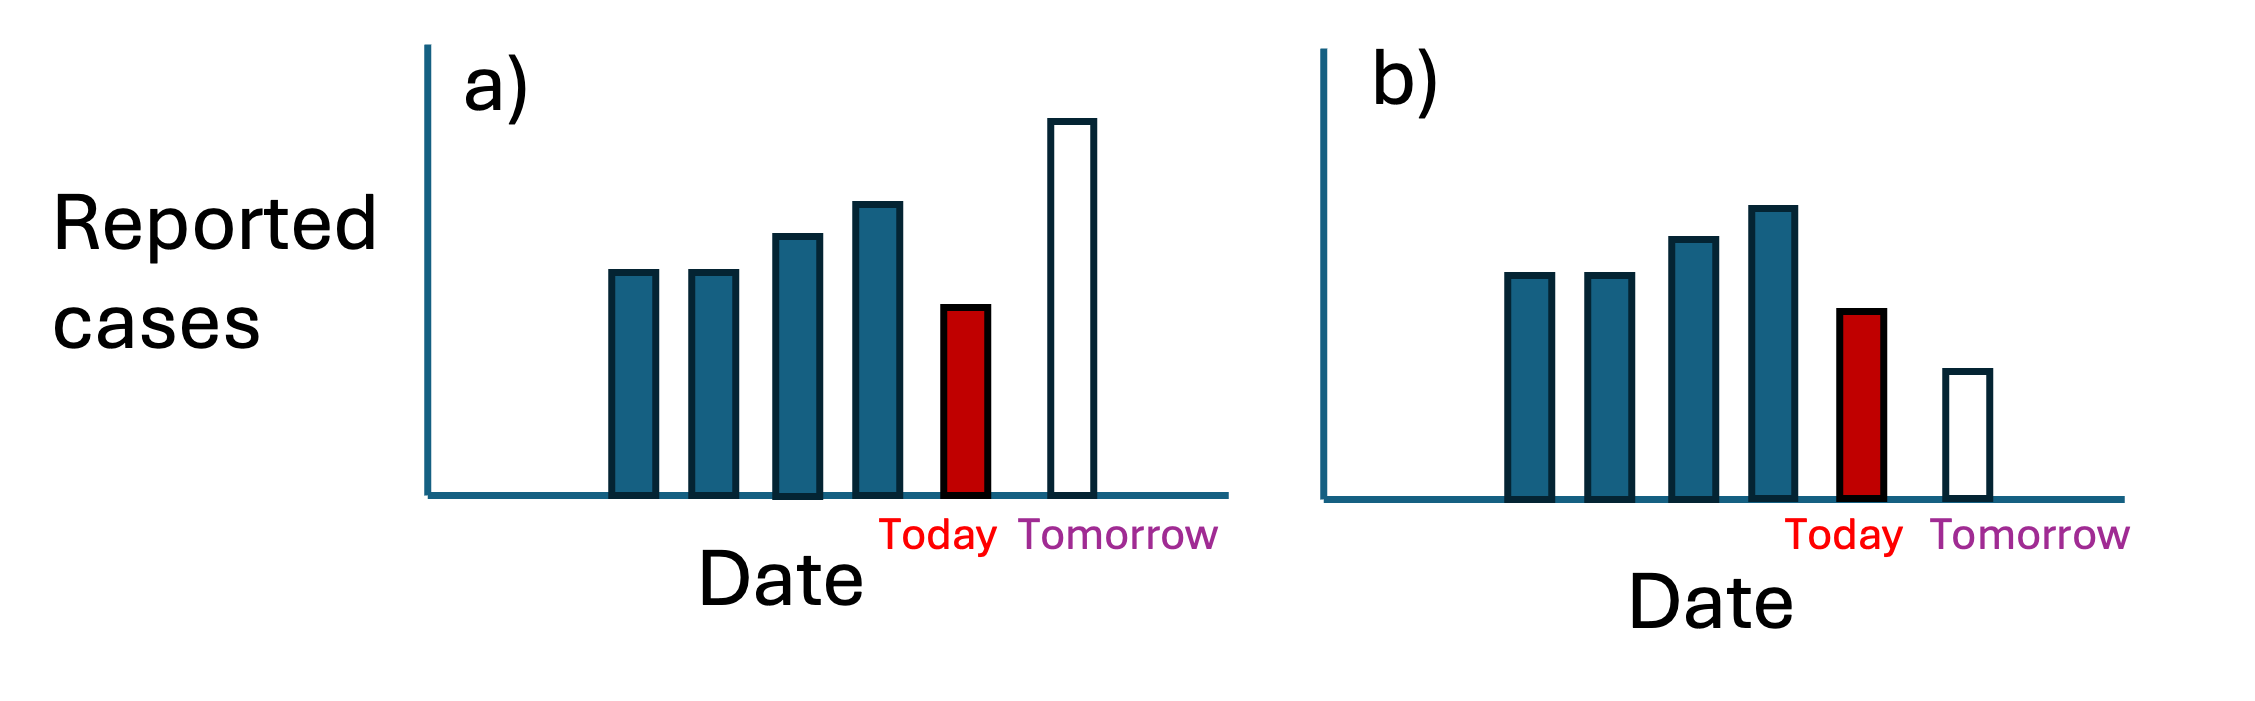
\includegraphics[width=0.8\linewidth,height=\textheight,keepaspectratio]{img/Tomorrow.png}

You may want to know, are cases tomorrow going to be a) higher than
today or b) lower than today. Just looking visually, either seems
plausible: in case a) perhaps today's cases are a outlier, and the true
trend will continue upwards, and in case b) perhaps today's cases are
not an outlier, and tomorrow's cases will be lower.

However the process that generates these new cases, i.e.~infection, has
already occurred in most cases. A more helpful question might be: Are
people still infecting other people in sufficient numbers that we can
expect cases to generally keep increasing? Reported cases are a lagging
indicator of the current state of disease transmission. If we understand
this dynamic, then we will be able to predict how many cases we expect
to be coming in the near future and if control measures are effectively
slowing transmission.

This is what the \textbf{effective reproductive number}, \(R(t)\), aims
to estimate. The reproductive number estimates the average number of
people an infectious individual will infect at time \(t\). This is
typically done daily. The reproductive number is estimated from case
count data like that shown in the plots above. But there is another
critical piece of information to indicate when reported cases might have
been infected. This is:

\textbf{How long does it take for an infected person to infect others?}
This is described by the generation interval. This can be summarized by
a mean which would give the average amount of time between an infector
and their infectee. But more often it is described by a statistical
distribution. For example, the infector of an infected individual would
have been infected 1 day prior with 30\% probability, 2 days prior with
40\% probability, or 3 days prior with probability.

The generation interval is central to estimating the reproductive
number. The generation interval can estimated by a number of methods,
including analyzing data of
\href{https://journals.lww.com/epidem/FullText/2009/05000/Estimation_of_the_Serial_Interval_of_Influenza.7.aspx?casa_token=ryVMHOD5AEgAAAAA:dTLXhhBPGA_sFo1yyON5_GDSwqV7cvMxb7p7FJAfHlO3OnpLfbTDLdgiWKNNz3_P4rQm18po9HSte9PtG_Sa0MQKRL0}{infector-infectee
pairs}.

Knowing \(R(t)\) can help you begin to make an informed guess as to the
current state of a disease outbreak and near term forecasts, as it has
the following values and interpretations \emph{at a specific point in
time}:

\begin{longtable}[]{@{}lll@{}}
\toprule\noalign{}
\endhead
\bottomrule\noalign{}
\endlastfoot
R(t) & Interpretation at time t & Outbreak is ... \\
\textless{} 1 & Each infected person infects \emph{on average} fewer
than one additional person & shrinking \\
= 1 & Each infected person infects \emph{on average} about one
additional person & stable \\
\textgreater{} 1 & Each infected person infects \emph{on average} more
than one additional person & growing \\
\end{longtable}

However, estimating \(R(t)\) is not straightforward, and is the subject
of a wealth of academic research and proliferation of software packages.
Guidance in choosing a choosing a method (and a package) is the purpose
of this website.

\subsection*{\texorpdfstring{How to choose a tool to estimate
\(R(t)\)}{How to choose a tool to estimate R(t)}}\label{how-to-choose-a-tool-to-estimate-rt}
\addcontentsline{toc}{subsection}{How to choose a tool to estimate
\(R(t)\)}

There has been a proliferation of software tools that make inference
about the current state of an infectious disease outbreak.

Important to keep in mind when choosing a tool to estimate \(R(t)\) is
this fact: \(R(t)\) is a \emph{latent} variable, which means
\emph{cannot be measured directly}. Instead, it can only be estimated
from observable variables (like reported case counts).

The ideal estimator of \(R(t)\) requires a list of the number of newly
\emph{infected} cases by infection date and the generation interval.
This is because we want to know about the state of disease based on when
people are infected, not when they report having symptoms. In reality we
usually only observe the new number of newly \emph{reported} cases and
can only estimate the serial interval, which is the time between symptom
onset of an infector-infectee pair. In this case the estimate of
\(R(t)\) will lag reality without some adjustments.

Each software package that estimates \(R(t)\) makes different
adjustments and assumptions about how these parameters relate, which
leads to variations in estimated \(R(t)\) \emph{even if the same input
data are used}. In addition, different packages require different levels
on input data to provide additional robustness in estimated outputs.

The purpose of this document

Therefore, the purpose of this document is to provide guidance about
which \(R(t)\) estimation software to choose for different analytical
goals. First, see our \href{simulation_tool.qmd}{Example outbreak} for
the different components of disease outbreak that can be modeled
differently. Next, see our \href{decisiontree.qmd}{Decision tool} for
how to choose software for different analytical goals.

\section*{Funding, authors, and
acknowledgements}\label{funding-authors-and-acknowledgements}
\addcontentsline{toc}{section}{Funding, authors, and acknowledgements}

\markright{Funding, authors, and acknowledgements}

This work is supported by CDC grant NU38FT000013.

The lead authors of this document are at Boston University in the School
of Public Health:

\begin{itemize}
\tightlist
\item
  Chad Milando, Laura White
\end{itemize}

Many additional co-authors contributed to this document including:

\begin{itemize}
\tightlist
\item
  Anne Cori, Brennan Klein, Katelyn Gostic, Alessandra Urbinati,
  Guillaume St-Onge, George Vega Yon, Kaitlyn Johnson, Christine
  Sangphet, \ldots{}
\end{itemize}

\bookmarksetup{startatroot}

\chapter*{Example outbreak}\label{example-outbreak}
\addcontentsline{toc}{chapter}{Example outbreak}

\markboth{Example outbreak}{Example outbreak}

\bookmarksetup{startatroot}

\chapter*{Decision matrix}\label{decision-matrix}
\addcontentsline{toc}{chapter}{Decision matrix}

\markboth{Decision matrix}{Decision matrix}

\(R(t)\) has two main uses:

\begin{enumerate}
\def\labelenumi{\arabic{enumi}.}
\tightlist
\item
  \textbf{Retrospective} understanding of the dynamics of historical
  outbreaks, and
\item
  \textbf{Real time tracking} ongoing infectious diseases.
\end{enumerate}

For 1, one might wish to understand the impact on transmission of
vaccines or non pharmaceutical interventions, such as masking or
physical distancing.

For real time tracking of ongoing infectious diseases, there is often
interest in determining if the current outbreak is getting worse, better
or staying the same. In this case, live dashboards are often used to
track \(R(t)\) as new data on diagnosed cases emerges. This is currently
done for COVID-19 and Influenza by the CDC and CA (add refs).

In either application, \textbf{delay distributions play a key role in
estimating \(R(t)\) for new infections.} You can use the decision tool
below to help choose which software package(s) may be right for your
application:

\begin{enumerate}
\def\labelenumi{\arabic{enumi}.}
\tightlist
\item
  Look first for the desired output that you want to produce
\item
  Then make a decision about whether you want to incorporate delay
  distributions.
\item
  Finally, estimate \(R(t)\) using the packages that are appropriate for
  your use case
\end{enumerate}

See below the table for the assessment framework used to decide which
packages to recommend.

\begin{tcolorbox}[enhanced jigsaw, opacityback=0, title=\textcolor{quarto-callout-note-color}{\faInfo}\hspace{0.5em}{Focus of this matrix}, leftrule=.75mm, toprule=.15mm, bottomrule=.15mm, coltitle=black, opacitybacktitle=0.6, toptitle=1mm, colframe=quarto-callout-note-color-frame, colback=white, rightrule=.15mm, colbacktitle=quarto-callout-note-color!10!white, titlerule=0mm, breakable, bottomtitle=1mm, arc=.35mm, left=2mm]

The table below focuses on \textbf{R packages} that esimate \(R(t)\)
using \textbf{reported cases}.

Future efforts include expanding this table to include
\textbf{alternative data sources} (e.g., wastewater) and packages in
\textbf{other coding languages} (e.g., Python). See the
\href{packages.qmd}{packages list} for an index of currently reviewed
packages.

\end{tcolorbox}

\begin{longtable}[]{@{}lcc@{}}
\caption{Decision matrix for choosing an R package for R(t)
estimation}\tabularnewline
\toprule\noalign{}
\endfirsthead
\endhead
\bottomrule\noalign{}
\endlastfoot
Desired output & Incorporates Delay distributions? & Package \\
\multirow{2}{=}{\ul{Forecasting}: what will R(t) be next week} & Yes &
\href{package_EpiNow2.html}{EpiNow2} \\
& No & \href{package_EpiInvert.html}{EpiInvert} \\
\multirow{2}{=}{\ul{Nowcasting}: what was R(t) in the past week} & Yes &
\textquotesingle{} \href{package_EpiNow2.html}{EpiNow2},
\href{package_epinowcast.html}{EpiNowcast},
\href{package_EstimateR.html}{EstimateR} \\
& No & \href{package_EpiLPS.html}{EpiLPS},
\href{package_EpiInvert.html}{EpiInvert} \\
\multirow{2}{=}{\ul{Historical}: what was R(t) over the past month} &
Yes & \href{package_EpiNow2.html}{EpiNow2},
\href{package_epinowcast.html}{EpiNowcast},
\href{package_EstimateR.html}{EstimateR} \\
& No & \href{package_EpiLPS.html}{EpiLPS},
\href{package_EpiInvert.html}{EpiInvert},
\href{package_RtEstim.html}{RtEstim},
\href{package_EpiEstim.html}{EpiEstim}, \href{package_R0.html}{R0} \\
\end{longtable}

\subsection*{Assessment framework}\label{sec-assessment}
\addcontentsline{toc}{subsection}{Assessment framework}

An objective comparison of the performance of the methods in these
packages would be highly complex, given the following challenges:

\begin{itemize}
\tightlist
\item
  These packages are really a combination of mathematical modeling,
  available data, and implementation. Any evaluation would have to
  disaggregate these features.
\item
  Some of the most widely-used packages are not accompanied with a
  peer-reviewed manuscript that describes or evaluates the theory behind
  modeling choices.
\item
  Each package contains a subset of the methods below for constraining
  \(R(t)\) in time, but with subtle variations in implementation and
  presentation that are often not well-documented and have large
  implications on evaluation metrics.
\item
  Some packages have not been recently updated, and even those that have
  are not maintained on Installation, instead leaving updates on a
  development version on GitHub.
\item
  Performance may vary widely considering additional factors like ease
  of implementation and computational time.
\item
  it also may be the case that some methods of temporal smoothing work
  better in some cases versus other (very low case counts, rapid
  changes)
\end{itemize}

Indeed, many published validation efforts are often not ``apples to
apples'', i.e., comparing two models that are using different amounts of
information in estimating R(t). For example, comparing a model that has
used only data before time before t to estimate R(t) versus a model that
uses the entire historical record to estimate R(t) at time t.

Instead, we present some quantifiable reflections on various aspects of
utilizing each package. :

\begin{longtable}[]{@{}lll@{}}
\caption{Assessment rubric}\tabularnewline
\toprule\noalign{}
\endfirsthead
\endhead
\bottomrule\noalign{}
\endlastfoot
Category & Notes & Metric \\
Features & & \\
Ability to nowcast/forecast & Does the package have functionality to
incorporate both right-truncated data from reporting delays and
forecasting of near-future cases and/or R(t) values & ☐ Yes/no \\
Incorporates delay distributions & Does the package have methodology for
incorporating delay distributions (e.g., transmission times,
administrative delays) & ☐ Yes/no \\
Estimates expected cases & Does the package provide an estimate of
expected cases and/or infections, or just R(t) & ☐ Yes/no \\
Communicates uncertainty & Does the package detail how uncertainty is
incorporated into presented outputs & ☐ Yes/no \\
Documentation & & \\
Documentation of package methods & Is there a written report (or
published manuscript) that describes the theory behind modeling choices
and/or implementation & ☐ Yes/no \\
Documentation of package implementation & Are there sufficiently
detailed vignettes that would permit a new user to implement key package
features & ☐ Yes/no \\
\end{longtable}

\part{Explanation of methods}

To aid with interpretation of package outputs, we summarize the
currently used inputs, data, methods and assumptions in \(R(t)\)
estimation across the following categories:

 \href{methods_introduction.qmd}{⎘}: How the relationship between
\(R(t)\) and infections is defined  \href{methods_distributions.qmd}{⎘}:
How \(R(t)\) is constrained using distributions for key variables
 \href{methods_time.qmd}{⎘}: How \(R(t)\) is constrained over time
 \href{methods_additionaldata.qmd}{⎘}: Additional data and distributions
that are used to constrain \(R(t)\)  \href{methods_inference.qmd}{⎘}:
Inference frameworks that are used to estimate \(R(t)\)

We limit the methods discussed here to those for estimating historical
to present-day \(R(t)\) values using \textbf{daily case count data},
where a case can be flexibly defined as an individual with a reported
positive test (either through healthcare-seeking behavior, routine
surveillance, or a hospital admission).

\subsection*{Other methods not discussed here
include:}\label{other-methods-not-discussed-here-include}
\addcontentsline{toc}{subsection}{Other methods not discussed here
include:}

\begin{itemize}
\tightlist
\item
  inference of \(R(t)\) exclusively from alternative data sources (e.g.,
  genetic data (Walker et al. 2013), behavioral data (Bokányi et al.
  2023), or viral loads in waste-water (Huisman et al. 2022)),
\item
  calculations from compartmental, agent-based models, or network
  Bettencourt and Ribeiro (2008).
\end{itemize}

We also limit the discussion to packages in the statistical software R
(R Core Team 2022), which may exclude some packages in other software
programs that combine many of the methodological considerations
discussed below (Yang et al. 2022).

We attempt to harmonize the mathematical choices between each package
using terminology from each.

\chapter*{\texorpdfstring{Relating infections to
\(R(t)\)}{Relating infections to R(t)}}\label{relating-infections-to-rt}
\addcontentsline{toc}{chapter}{Relating infections to \(R(t)\)}

\markboth{Relating infections to \(R(t)\)}{Relating infections to
\(R(t)\)}

\subsubsection*{Overview}\label{overview-1}
\addcontentsline{toc}{subsubsection}{Overview}

There are two primary classes methods of estimating \(R(t)\) from case
count data that are used in most R software packages.

\begin{enumerate}
\def\labelenumi{(\arabic{enumi})}
\item
  The first class of methods assumes there is a formulaic relationship
  between infections and reproduction number, a relationship known as
  the renewal equation (Fraser 2007). These infections are then assumed
  to result in (some fraction of) the observed cases.
\item
  A second class of methods involves empirically calculating a quantity
  that approximates the latent quantity represented by a reproduction
  number by fitting a curve to the case count time-series and finding
  the time-varying slope in log space (and then performing other
  transformations). Empirical calculations are discussed in detail below
  in our examination of ways in which \(R(t)\) is constrained over time.
\end{enumerate}

\section*{Renewal equation estimates of
R(t)}\label{renewal-equation-estimates-of-rt}
\addcontentsline{toc}{section}{Renewal equation estimates of R(t)}

\markright{Renewal equation estimates of R(t)}

The renewal equation relates \(R(t)\) and infections on day \(t\),
\(I(t)\), using a third parameter known as the generation interval. The
generation interval, \(ω\), is the time between infection in the
infector and infection in the infectee, and assuming independence is the
linear combination of incubation time, the time between infection and
symptom onset in an individual, and transmission time, the time between
symptom onset in the infector and infection of the infectee (Lehtinen et
al. 2021).

A similar parameter to the generation interval is the serial interval,
which is the time between symptom onset in the infector and symptom
onset in the infectee. The serial interval and generation interval are
interchangeable if the incubation time is independent from the
transmission time, and some formulations of the renewal equation use
generation interval.

In this paper we use the generation interval \(ω\) described by a
probability mass function with non-zero values from day 1 (assuming that
disease incubation takes at least 1 day) to a maximum day \(s\), i.e.,
the longest interval between symptom onset in infector and infectee.

Taking care to note that \(R(t)\) is undefined on day 0 since there has
been no transmission yet (and assuming the initial infections are
\(I(0)\)), the formulation of the renewal equation is thus:

\[
I(t) = R(t) \sum_{i = \max(1, t - s + 1)}^{t} \omega(i) \, I(t - i)
\]

For brevity, we write the inner sum of (Eq.1) as:

\[
Λ(t) =  \sum_{i = \max(1, t - s + 1)}^{t} \omega(i) \, I(t - i)
\]

The assumptions of this formulation, as per Green et al. (2022), are
that incident infections can be described deterministically within each
window of \([t-s+1,t]\) and that the generation interval distribution
does not change over the modeling time.

A common reframing of the renewal equation is to equate \(R(t)\) with an
exponential growth rate, \(r\). Under specific conditions and within a
small time window (\([t-s+1,t]\)), infections can be assumed to grow
exponentially at a constant rate \(r\) Wallinga and Lipsitch (2006).
Using the time window \([t- s+1,t]\) and assuming some initial
infections \(k\), \(R(t)\) for \([t- s+1,t]\) can be inferred from only
\(r\) and \(ω\):

\[
I(t)=ke^rt
\] \[
R(t)= [\sum_{i = \max(1, t - s + 1)}^{t} \omega(i) \, e^{-ri}]^{-1}        
\]

Again, we will omit the writing the bounds for time in remaining
formulae. A single \(R(t)\) value, say \(R_0\), can also be put in the
form of an infection attack rate, \(z\) Musa et al. (2020), or in the
final size equation Ma and Earn (2006), to estimate the proportion of
all individuals that were affected by a disease with this \(R_0\):

\[
z=1-exp⁡(-R_0  z)                   
\]

The attack rate function and others are implemented in the package
\href{package_epigrowthfit.qmd}{epigrowthfit}. The major difference
between calculating \(R(t)\) from a renewal equation or an exponential
growth rate equation is whether \(I(t)\) is used. If for a given time
window both r and ω can be estimated independently, then \(R(t)\) can be
inferred without infection data. Otherwise, infection data are needed to
estimate \(R(t)\).

\subsection*{\texorpdfstring{Solving for
\(R(t)\)}{Solving for R(t)}}\label{solving-for-rt}
\addcontentsline{toc}{subsection}{Solving for \(R(t)\)}

\begin{tcolorbox}[enhanced jigsaw, opacityback=0, title=\textcolor{quarto-callout-warning-color}{\faExclamationTriangle}\hspace{0.5em}{Solving for \(R(t)\)}, leftrule=.75mm, toprule=.15mm, bottomrule=.15mm, coltitle=black, opacitybacktitle=0.6, toptitle=1mm, colframe=quarto-callout-warning-color-frame, colback=white, rightrule=.15mm, colbacktitle=quarto-callout-warning-color!10!white, titlerule=0mm, breakable, bottomtitle=1mm, arc=.35mm, left=2mm]

Using the renewal equation and given that \(I(t)\) and \(ω\) are known,
\(R(t)\) can be solved for algebraically starting with R(t=1) and
iterating forwards in time. However, this will produce highly volatile
estimates of \(R(t)\) that recover the incidence curve directly.

\end{tcolorbox}

Solving directly for \(R(t)\) at every timestep is undesirable for
several reasons:

\begin{itemize}
\tightlist
\item
  real-world infectivity likely does not vary dramatically from day to
  day
\item
  and real-world infection data are rarely complete, especially in an
  emerging epidemic, meaning that a certain amount of uncertainty must
  be incorporated into any estimation framework.
\item
  In addition, infection incidence, \(I(t)\), are the data of interest
  but it is impossible to observe, so many calculations instead may use
  the observed reported cases, \(C(t)\), which requires some additional
  processing to incorporate into calculations of \(R(t)\).
\end{itemize}

Therefore, a variety of constraints on \(R(t)\) are added in the
inferential process: using distributions on key variables, placing
restrictions on how \(R(t)\) varies through time, and with additional
data sources and delay distributions. These choices dictate which
estimation framework is used, which can add additional constraints.

\section*{\texorpdfstring{Empirical estimates of
\(R(t)\)}{Empirical estimates of R(t)}}\label{empirical-estimates-of-rt}
\addcontentsline{toc}{section}{Empirical estimates of \(R(t)\)}

\markright{Empirical estimates of \(R(t)\)}

In contrast to models that assume that renewal equation defines the
relationship between infections and \(R(t)\), smoothing or regression
models calculate time-varying \(R(t)\) directly from slope of the log of
the infections time-series. Using this method, the relationship between
\(R(t)\) and infections is empirically defined, being only constrained
by the smoothing parameters of curve fit to infections data. Several R
packages contain methods for this type of smoothing, e.g.,
\href{package_EpiLPS.qmd}{EpiLPS}, \href{package_EpiNow2.qmd}{EpiNow2}

\chapter*{Distributions for key
variables}\label{distributions-for-key-variables}
\addcontentsline{toc}{chapter}{Distributions for key variables}

\markboth{Distributions for key variables}{Distributions for key
variables}

\section*{Distributions for key
variables}\label{distributions-for-key-variables-1}
\addcontentsline{toc}{section}{Distributions for key variables}

\markright{Distributions for key variables}

A primary component of constraining \(R(t)\) is how distributions are
used to constrain key variables in \(R(t)\) estimation: for \(I(t)\),
\(ω\), and for \(R(t)\) itself.

Assuming some prior distributions for \(R(t)\) and the generation
interval permit an analytical solution for the posterior distribution of
\(R(t)\), as in \href{package_EpiEstim.qmd}{EpiEstim}. These simplifying
assumptions greatly constrain the space of potential \(R(t)\) and thus
calculation times are relatively fast.

Other software packages, such as \href{package_EpiNow2.qmd}{EpiNow2},
have more flexibility at the cost of somewhat higher computational
runtime and resources.

\section*{Distributions used to define new offspring from
cases}\label{distributions-used-to-define-new-offspring-from-cases}
\addcontentsline{toc}{section}{Distributions used to define new
offspring from cases}

\markright{Distributions used to define new offspring from cases}

Another primary component of constraining \(R(t)\) is how distributions
are used to define the next generation of infections, or \(I(t)\) from
\(I(t-1)\).

The renewal equation provides a mechanism for estimating the next batch
of infectees that occur due to transmission from the current round of
infectors, a branching process. For \(time = t-1\) the \(I(t)\)
calculated in the renewal equation provides the expected value for a
draw from a discrete distribution, the value of which represents the
next generation of infectees.

The discrete distribution chosen is commonly a \textbf{Poisson
distribution} (in which the mean and variance parameter \(λ(t)=I(t)\)).
Thus, using this constraint, the time-series of \(I(t)\) represents
draws from a series of Poisson distributions with means of \(λ(t)\).

Alternatively, a \textbf{Negative Binomial distribution} can be used
(with a mean parameter again equal to \(I(t)\)), although this requires
additionally fitting the size parameter (roughly, the spread of the
distribution) to account the infectee distribution being
``over-dispersed''.

Importantly, if additional delay distributions are included in the
process of estimating \(R(t)\), the parameter that distributions are
being used to estimate for the next generation may change, see reference
for \href{package_EpiNow2.qmd}{EpiNow2} for more details.

\chapter*{\texorpdfstring{Constraining \(R(t)\) over
time}{Constraining R(t) over time}}\label{constraining-rt-over-time}
\addcontentsline{toc}{chapter}{Constraining \(R(t)\) over time}

\markboth{Constraining \(R(t)\) over time}{Constraining \(R(t)\) over
time}

\subsubsection*{Overview}\label{overview-2}
\addcontentsline{toc}{subsubsection}{Overview}

The largest variety in constraints of \(R(t)\) exists in methods that
impose structure on how \(R(t)\) varies with time. Each method confers
various assumptions and implications for resulting estimates of
\(R(t)\), and new methods represent a large area of innovation with
regards to real-time infectious disease modeling. With these
constraints, we can make inference from sampled case-count data as a
signal of unobserved infections in the larger unobserved population.

\section*{Fixed sliding windows}\label{sec-fixedwindow}
\addcontentsline{toc}{section}{Fixed sliding windows}

\markright{Fixed sliding windows}

A straightforward method of imposing structure on \(R(t)\) over time
involves constraining \(R(t)\) to be drawn from the same distribution
within moving time subsets, called sliding windows.

We add the prefix of ``fixed-size'' to distinguish from methods that may
adapt the size of the sliding window over time.

Consider the scenario where I(t) are drawn from a series of Poisson
distributions and where R(t) are drawn from a series of Gamma
distributions. Using a sliding window size, τ, of 5 days: * R(t) on days
2 to 6 are assumed to be drawn from the Gamma distribution with
parameters \(a_1\) and \(b_1\), * R(t) on days 3 to 7 are drawn from a
Gamma distribution with parameters a\_2 and b\_2, and so on.

In the above scenario, days 3 through 6 are in both windows and thus
will be values that could be reasonably drawn from Gamma distributions
with either \(a_1\) and \(b_1\) or \(a_2\) and \(b_2\).

Using an assumption of Gamma distributions for the prior distribution of
ω and R(t), Cori et. al.~(2013)18 analytically derived a posterior
distribution R(t) using fixed-size sliding windows, which has the
following directly calculated (rather than inferred) mean and
coefficient of variation of \(R(t)\):

\[
E[R(t)]=[a+ ∑_(i=max⁡(1,   t-τ))^t▒I(i) ]/[1/b+∑_(i=max⁡(1,   t-τ))^t▒Λ(i) ]  
\]

\[
C.V.[R(t)]=[a+ ∑_(i=max⁡(1,   t-τ))^t▒I(i) ]^(-1)               (Eq.7)
\]

Thus, sliding windows with larger τ improve the stability of the
estimate of R(t) over smaller τ because the coefficient of variation of
R(t) decreases as number of infections increases (see Web Appendix 1 of
Cori et. al., 2013).18 Sliding windows are a key feature of EpiEstim.21

There are limitations of this derived sliding window approach,
articulated well in Gostic et. al., (2020)1 and summarized here:

\begin{itemize}
\item
  There is no posterior distribution for the expected value of incidence
  In the fixed size sliding window approach, τ must be explicitly
  defined prior to inference.
\item
  Shorter τ will lead to quicker response but more variable estimates of
  R(t), which increases the risk of over-fitting. At the extreme, if the
  τ is set to 1 day, the resulting R(t) will recover exactly the
  infection data.
\item
  In addition, there is debate in the literature about where in time the
  estimate of R(t) for each window should go: Gostic et. al., (2020)1
  recommends using the midpoint of each sliding window rather than time
  t.
\item
  The choice of both τ and the location of the estimate of R(t) within
  each window results in gaps in predictions for R(t), barring other
  modifications: at the end of the modeling period to account for
  reporting delays or time between the midpoint of τ and the end of τ,
  and at the beginning of the time period to allow for enough cases to
  materialize. Web Appendix 4 of Cori. et. al (2013) gives the following
  recommendation for when to calculate R(t): ``Overall, we suggest
  starting estimating once those three criteria are fulfilled: at least
  after , at least after one mean serial interval, and when at least 12
  cases have been observed since the beginning of the epidemic.'' The
  default recommendation for τ is one week (7 days);18
\end{itemize}

\subsection*{Accumulated Prediction Error (APE)
framework}\label{sec-ape}
\addcontentsline{toc}{subsection}{Accumulated Prediction Error (APE)
framework}

Alternatively the package \href{package_APEestim.qmd}{APEestim}
integrates with \href{package_EpiEstim.qmd}{EpiEstim} to propose a
non-default choice of τ that minimizes one-step-ahead prediction errors
(Parag and Donnelly (2020)).

In APEestim, Parag et al.~adapt an approximation known as the
accumulated prediction error (APE) to identify the window length best
justified by the available epi-curve, k*, to opitmizing the window
length k.

\subsection*{Modification via variational method}\label{sec-var}
\addcontentsline{toc}{subsection}{Modification via variational method}

In \href{package_EpiInvert.qmd}{EpiInvert}

\subsection*{Disaggregation}\label{sec-disagg}
\addcontentsline{toc}{subsection}{Disaggregation}

Package \href{package_ern.qmd}{ern}

\section*{Random walk}\label{sec-randomwalk}
\addcontentsline{toc}{section}{Random walk}

\markright{Random walk}

Another method of constraining how \$R(t)4 evolves in time is to define
the relationship between R(t), infections, and time in a random walk or
auto-regressive framework. In this framework, there are latent or
unobserved variables, e.g., R(t), that depend on observed variables,
e.g., I(t) via the renewal equation, and the evolution of the unobserved
variables through time can be parameterized. The auto-regressive
component means that the current value of R(t) is correlated via some
mechanism with R(t-1) (and potentially other past values). The packages
epidemia23 and EpiNow2 contain an implementations of a random walk
procedure that look generally as follows:

f(R(t))=f(R(t-1))+N(0,σ\_R) (Eq.8) σ\_R \textasciitilde{}
HalfNormal(ρ,φ) (Eq.9)

The random walk implies that adjacent R(t) values may be drawn from
similar or even the same distribution, and would be correlated in time
based on previous values. The variables ρ and φ are hyperparameters. The
function f can be a transformation of R(t), e.g.~in log space as in
EpiNow2 to correct for the skewness of R(t), provide a variable that is
more Gaussian, provide a variable that obeys the properties that we
expect from R(t) (i.e., is non-negative), and aid in interpretability.
The function f in epidemia contains more layers for pooled effects and
group-level variables.

\section*{Filtering}\label{sec-filtering}
\addcontentsline{toc}{section}{Filtering}

\markright{Filtering}

Filtering is another way that R(t) is constrained in common packages.
Filtering means {[}\ldots{]}. One way that a filter could be implemented
is in a Hidden Markov Model.24 A simple forward-looking linear filter
for R(t) in an Hidden Markov Model might look as follows, with a tuning
parameter (η) to influence the amount that R(t) can vary between
time-steps and a standard white noise component (ϵ):

R(t)=R(t-1)+(η√(R(t-1) ))ϵ(t-1) (Eq.10)

The package EpiFilter25 implements a two-stage filtering and smoothing
method for estimating R(t). A key innovation of EpiFilter is that the
states of historical R(t) are constrained to a predefined set of values;
this dramatically reduces calculation time. The smoothing stage refines
estimates of R(t) by incorporating future incidence, in this way using
all available data in estimates of historical R(t). These modeling steps
help avoid R(t) instability when infections are low and instability at
the beginning and (more importantly) the end of the modeling period.

Another way that filtering can be implemented is across the entire R(t)
time-series.

\begin{verbatim}
RtEstim:28 https://dajmcdon.github.io/rtestim/articles/delay-distributions.html

We propose a discrete spline-based approach, RtEstim, that solves a convex optimization problem—Poisson trend filtering—using the proximal Newton method. It produces a locally adaptive estimator for effective reproduction number estimation with heterogeneous smoothness.28
EpiLPS:29
\end{verbatim}

In EpiFilter, RtEstim, and EpiLPS, each R(t) estimated in this way thus
contains information about past and pending infections, e.g., for
R(t=i), the smoothing step will affect R(t=i) using information from
0\textless i≤t\_max. This complicates comparisons to outputs from other
methods that only use historical information to estimate R(t), e.g.,
estimates for R(t=i) containing only information from t\textless i.

\section*{Gausian Process models}\label{sec-gaussianprocess}
\addcontentsline{toc}{section}{Gausian Process models}

\markright{Gausian Process models}

Gaussian Process models26 are a more flexible method of constraining the
evolution of R(t) in time than the methods discussed thus far (in fact,
a random-walk process can be thought of as a simplified case of Gaussian
Process model). In Gaussian Process modeling, a family of basis
functions are fit to available data, permitting inference about
continuous processes without needing to a priori define where inflection
points occur. The core of Gaussian Process operations is a kernel, which
is used to assess the similarity between input vectors, say x and
x\^{}'. There are many options for potential kernels, and each contains
different hyperparameters that are used to control the amount of
smoothing that is enforced, as well as other factors. One such choice is
the squared exponential kernel:

k(x,x\^{}' )=α\^{}2 exp⁡{[}-(x-x\^{}' )\textsuperscript{2/(2l}2 ){]}
(Eq.10)

In this kernel, the hyperparameters are the length scale, l, which
controls the smoothness of the model, and the magnitude, α, which
controls the range of values used in the fitting process. These
parameters can be given prior distributions and fit using optimization.
EpiNow2 uses contains options to use Gaussian Process models to control
how R(t) in time. As one example, the relationship between first
difference values of R(t) can be constrained using a zero-mean Gaussian
Process model with the above kernel as the covariance function:

\begin{verbatim}
    log⁡〖R(t)=log⁡R(t-1)+ GP(0,k(R(t),〖R(t〗^')))〗       (Eq.11)
    
\end{verbatim}

The advantage of Gaussian Process models is that R(t) is enforced to
change smoothly in time using Eq.10. Limitations include complexity and
computational time: Gaussian Process models have a computational
complexity of O(n\^{}3) for n observations.27 Although EpiNow2 in
practice implements faster approximations of Gaussian Process models,27
in general Gaussian Process runtimes and required computational
resources are considerable as compared to other methods.

\chapter*{Additional data}\label{additional-data}
\addcontentsline{toc}{chapter}{Additional data}

\markboth{Additional data}{Additional data}

Estimates of R(t) can also be improved using additional data. , you can
beef up the calculation by including other pieces of information about
counts.

\section*{Reconstruction of missing
data}\label{reconstruction-of-missing-data}
\addcontentsline{toc}{section}{Reconstruction of missing data}

\markright{Reconstruction of missing data}

Extending EpiEstim • The package bayEStim30 also extends EpiEstim o Our
method extends that of Cori et al (2013), adding Bayesian imputation of
missing symptom onset dates, imputation of infection times using an
external estimate of the incubation period, and an adjustment for
reporting delay. • Tenglong's work31 and the accompanying package
WhiteLabRt32 use the sliding window approach to estimating missing
reporting delay information from line-list data (originally implemented
as a Gibbs sampler, later updater to STAN). • The package estimateR
involves estimating missing count data using smoothing {[}confirm{]}.33

• Does EpiNow2 do this?

\href{package_Epidemia.qmd}{Epidemia}: 23 . We introduce a Bayesian
mechanistic model linking the infection cycle to observed deaths,
inferring the total population infected (attack rates) as well as Rt.

\section*{Delay distributions}\label{delay-distributions}
\addcontentsline{toc}{section}{Delay distributions}

\markright{Delay distributions}

Importantly, the definition of R(t) is linked to the data that are being
used, so models that calculate a similar quantity as R(t) but instead
from infections, symptom onset, or reports are important quantities but
differ in definition from the instantaneous reproduction number R(t) as
defined throughout the literature. sometimes R(t) is calculated directly
from reported case data and then shifted backwards by a delay
distribution, whereas other times R(t) is calculated from inferred dates
of infection using reported case data.

Reporting delay, Onset delays etc Delay PMFs that you can pass in series
which have cascading impacts.

\begin{verbatim}
EpiNow2 has this:
Our estimates overcome some of the limitations of naive implementations that derive estimates for the reproduction number directly from numbers of reported cases without adjusting (or with only partial adjustments) for the delay from infection to symptom onset or from onset to notification. 
Our approach also incorporates multiple sources of uncertainty that if excluded can bias estimates.

EpiFilter was also recently generalized to incorporate hetereogeonous transmission rates and reporting delays.34
\end{verbatim}

Several packages have been created to extend
\href{package_EpiEstim.qmd}{EpiEstim} to use delay distributions:

\begin{itemize}
\tightlist
\item
  \href{package_bayEStim.qmd}{bayEStim}: Our method extends that of Cori
  et al (2013), adding Bayesian imputation of missing symptom onset
  dates, imputation of infection times using an external estimate of the
  incubation period, and an adjustment for reporting delay.
\item
  \href{package_EstimateR.qmd}{estimateR} involves combining various
  delay distributions with \href{package_EpiEstim.qmd}{EpiEstim}
\item
  \href{package_EpiInvert.qmd}{EpiInvert} also has methods for including
  delay disributions with \href{package_EpiEstim.qmd}{EpiEstim}
\end{itemize}

\section*{Clinical data
distributions}\label{clinical-data-distributions}
\addcontentsline{toc}{section}{Clinical data distributions}

\markright{Clinical data distributions}

Again, some packages just modify EpiEstim:

\begin{itemize}
\tightlist
\item
  The \href{package_ern.qmd}{ern} package ultimately uses the
  \href{package_EpiEstim.qmd}{EpiEstim} package for the core of the
  computation as \href{package_EpiEstim.qmd}{EpiEstim} already provides
  a robust and one of the fastest implementations of well-tested
  estimation algorithms. However, \href{package_ern.qmd}{ern} wraps
  complex and critical features for estimating from real-world clinical
  and wastewater data that have not all been implemented in any one
  existing package for estimation
\end{itemize}

Here, we present the library \href{package_ern.qmd}{ern} to address the
gaps identified above, specifically: o to disaggregate the clinical
reports into a shorter time unit to enable estimation of using an
intrinsic generation interval on a useful timescale; o to provide a
framework to estimate from wastewater data, consistent with an
estimation based on clinical data; o to provide a user-friendly
interface geared at public-health practitioners that may have limited
proficiency in the programming language; o to perform an efficient and
rapid estimation.

\section*{Linear predictor model
components}\label{linear-predictor-model-components}
\addcontentsline{toc}{section}{Linear predictor model components}

\markright{Linear predictor model components}

ViaEpidemia School closures etc

EpiFusion:37 We propose a model of Rt that estimates outbreak
trajectories conditional upon both phylodynamic (time-scaled trees
estimated from genetic sequences) and epidemiological (case incidence)
data.

\chapter*{Inference frameworks}\label{inference-frameworks}
\addcontentsline{toc}{chapter}{Inference frameworks}

\markboth{Inference frameworks}{Inference frameworks}

Finally there are different ways of acutally calculating the numbers
once you have the theory lined up.

\section*{Bayesian optimization}\label{bayesian-optimization}
\addcontentsline{toc}{section}{Bayesian optimization}

\markright{Bayesian optimization}

 Assumes a distribution --\textgreater{} solved analytically • EpiEstim
o restricted set of GI options (gamma?) enables analytical solve for the
posterior estimate of R(t) which is also a Gamma, using conjugate priors

 Doesn't assume a distribution of R(t) or I(t) --\textgreater{} Uses
MCMC • EpiNow2, implemented in STAN • Hierarchical NUTS

\section*{MaxLiklihood optimization}\label{maxliklihood-optimization}
\addcontentsline{toc}{section}{MaxLiklihood optimization}

\markright{MaxLiklihood optimization}

• Frequentist o RtEstim

Wallinga, J., and P. Teunis. ``Different Epidemic Curves for Severe
Acute Respiratory Syndrome Reveal Similar Impacts of Control Measures.''
American Journal of Epidemiology 160,no. 6 (2004): 509. • \^{} this has
the likelihood calculation in it

One of the most widely used methods for estimating time-varying
reproduction number is a maximum likelihood-based approach \{White,
2008\}. • White LF, Pagano M. A likelihood-based method for real-time
estimation of the serial interval and reproductive number of an
epidemic. Stat Med 2008; 27(16): 2999--3016.

\chapter*{Open research questions}\label{open-research-questions}
\addcontentsline{toc}{chapter}{Open research questions}

\markboth{Open research questions}{Open research questions}

\begin{itemize}
\tightlist
\item
  Need to add a page of existing research questions

  \begin{itemize}
  \tightlist
  \item
    sub-regional or pooling \ldots{}
  \item
    other stuff, i think you had a list of this somehwere
  \end{itemize}
\end{itemize}

\part{Packages}

\chapter*{APEestim}\label{apeestim}
\addcontentsline{toc}{chapter}{APEestim}

\markboth{APEestim}{APEestim}

\begin{longtable}[]{@{}
  >{\raggedright\arraybackslash}p{(\linewidth - 2\tabcolsep) * \real{0.2000}}
  >{\raggedright\arraybackslash}p{(\linewidth - 2\tabcolsep) * \real{0.8000}}@{}}
\toprule\noalign{}
\endhead
\bottomrule\noalign{}
\endlastfoot
REF & Parag and Donnelly (2020) \\
Docs & None \\
Github &
\href{https://github.com/kpzoo/model-selection-for-epidemic-renewal-models}{Github} \\
Last commit & Feb 12, 2021 \\
Installation & None, this is code to augment
\href{package_EpiEstim.qmd}{EpiEstim} \\
\end{longtable}

\subsection*{Description}\label{description}
\addcontentsline{toc}{subsection}{Description}

Copied from the developer site

\href{package_APEestim.qmd}{APEestim} estimates the time-varying
reproduction number on cases by date of infection (using a similar
approach to that implemented in \href{package_EpiEstim.qmd}{EpiEstim}).

The quality of this estimate is highly dependent on the size of a
smoothing window (k) that is employed. This code presents a method for
optimally selecting k in a manner that balances reliable R(t) estimation
with short-term forecasts of incidence. This method is based on the
accumulated prediction error (APE) idea from information theory.

\subsection*{Methods}\label{methods}
\addcontentsline{toc}{subsection}{Methods}

This package aims to improve upon the limitation of
\hyperref[sec-fixedwindow]{fixed sliding windows}, specifically by
optimizing the choice of the window size in an \hyperref[sec-ape]{APE
Framework}.

\subsection*{Assessment}\label{assessment}
\addcontentsline{toc}{subsection}{Assessment}

\begin{longtable}[]{@{}
  >{\raggedright\arraybackslash}p{(\linewidth - 2\tabcolsep) * \real{0.4000}}
  >{\raggedright\arraybackslash}p{(\linewidth - 2\tabcolsep) * \real{0.6000}}@{}}
\toprule\noalign{}
\endhead
\bottomrule\noalign{}
\endlastfoot
Features & \\
Ability to nowcast/forecast & No \\
Incorporates delay distributions & No \\
Estimates expected cases & No \\
Communicates uncertainty & Yes \\
Validation & \\
Documentation of package methods & Yes \\
Documentation of package implementation & No \\
\end{longtable}

\subsection*{Sample Code}\label{sample-code}
\addcontentsline{toc}{subsection}{Sample Code}

See
\href{https://github.com/kpzoo/model-selection-for-epidemic-renewal-models/blob/master/apeExamples.R}{this
file} in the Github repo.

\chapter*{bayEstim}\label{bayestim}
\addcontentsline{toc}{chapter}{bayEstim}

\markboth{bayEstim}{bayEstim}

\begin{longtable}[]{@{}
  >{\raggedright\arraybackslash}p{(\linewidth - 2\tabcolsep) * \real{0.2000}}
  >{\raggedright\arraybackslash}p{(\linewidth - 2\tabcolsep) * \real{0.8000}}@{}}
\toprule\noalign{}
\endhead
\bottomrule\noalign{}
\endlastfoot
REF &
\href{https://www.medrxiv.org/content/10.1101/2020.09.19.20198028v1}{Lytras
et al.~preprint} \\
Docs & None \\
Github &
\href{https://github.com/thlytras/bayEStim}{github.com/thlytras/bayEStim} \\
Last commit & Aug 3, 2020 \\
Installation & None \\
\end{longtable}

\subsection*{Brief description}\label{brief-description}
\addcontentsline{toc}{subsection}{Brief description}

Package never submitted to CRAN, no further action taken

\chapter*{earlyR}\label{earlyr}
\addcontentsline{toc}{chapter}{earlyR}

\markboth{earlyR}{earlyR}

\begin{longtable}[]{@{}
  >{\raggedright\arraybackslash}p{(\linewidth - 2\tabcolsep) * \real{0.2000}}
  >{\raggedright\arraybackslash}p{(\linewidth - 2\tabcolsep) * \real{0.8000}}@{}}
\toprule\noalign{}
\endhead
\bottomrule\noalign{}
\endlastfoot
REF & None \\
Docs &
\href{https://www.repidemicsconsortium.org/earlyR/articles/earlyR.html}{repidemicsconsortium.org/earlyR/articles/earlyR.html} \\
Github &
\href{https://github.com/reconhub/earlyR}{github.com/reconhub/earlyR} \\
Last commit & October 27, 2020 \\
Installation &
\href{https://cran.r-project.org/web/packages/earlyR/index.html}{CRAN} \\
\end{longtable}

\subsection*{Brief description}\label{brief-description-1}
\addcontentsline{toc}{subsection}{Brief description}

Copied from the developer site

Implements a simple, likelihood-based estimation of the reproduction
number (R0) using a branching process with a Poisson likelihood. This
model requires knowledge of the serial interval distribution, and dates
of symptom onsets. Infectiousness is determined by weighting R0 by the
probability mass function of the serial interval on the corresponding
day. It is a simplified version of the model introduced by Cori et al.
(2013).

\subsection*{Methods}\label{methods-1}
\addcontentsline{toc}{subsection}{Methods}

This package does not constrain R in time, instead this is meant to
predict a single R value (R0) and then uses this to nowcast and forecast
cases.

\subsection*{Assessment}\label{assessment-1}
\addcontentsline{toc}{subsection}{Assessment}

\begin{longtable}[]{@{}
  >{\raggedright\arraybackslash}p{(\linewidth - 2\tabcolsep) * \real{0.4000}}
  >{\raggedright\arraybackslash}p{(\linewidth - 2\tabcolsep) * \real{0.6000}}@{}}
\toprule\noalign{}
\endhead
\bottomrule\noalign{}
\endlastfoot
Features & \\
Ability to nowcast/forecast & Yes \\
Incorporates delay distributions & No \\
Estimates expected cases & Yes \\
Communicates uncertainty & Yes \\
Validation & \\
Documentation of package methods & No \\
Documentation of package implementation & Yes \\
\end{longtable}

\subsection*{Sample Code}\label{sample-code-1}
\addcontentsline{toc}{subsection}{Sample Code}

\href{https://cran.r-project.org/web/packages/earlyR/vignettes/earlyR.html}{This
vignette} gives a basic example of usage

\chapter*{Epidemia}\label{epidemia}
\addcontentsline{toc}{chapter}{Epidemia}

\markboth{Epidemia}{Epidemia}

\begin{longtable}[]{@{}
  >{\raggedright\arraybackslash}p{(\linewidth - 2\tabcolsep) * \real{0.2000}}
  >{\raggedright\arraybackslash}p{(\linewidth - 2\tabcolsep) * \real{0.8000}}@{}}
\toprule\noalign{}
\endhead
\bottomrule\noalign{}
\endlastfoot
REF & Flaxman et al. (2020) \\
Docs &
\href{https://imperialcollegelondon.github.io/epidemia/index.html}{imperialcollegelondon.github.io/epidemia} \\
Github &
\href{https://github.com/ImperialCollegeLondon/epidemia}{github.com/ImperialCollegeLondon/epidemia} \\
Last commit & Feb 12, 2021 \\
Installation & Broken, see below \\
\end{longtable}

\subsection*{Brief description}\label{brief-description-2}
\addcontentsline{toc}{subsection}{Brief description}

This package
\href{https://github.com/ImperialCollegeLondon/epidemia/issues/67}{cannot
currently be installed} so no further analysis is provided at this time

\chapter*{EpiEstim}\label{epiestim}
\addcontentsline{toc}{chapter}{EpiEstim}

\markboth{EpiEstim}{EpiEstim}

\begin{longtable}[]{@{}
  >{\raggedright\arraybackslash}p{(\linewidth - 2\tabcolsep) * \real{0.2000}}
  >{\raggedright\arraybackslash}p{(\linewidth - 2\tabcolsep) * \real{0.8000}}@{}}
\toprule\noalign{}
\endhead
\bottomrule\noalign{}
\endlastfoot
REF & Cori et al. (2013), Nash et al. (2023) \\
Docs &
\href{https://mrc-ide.github.io/EpiEstim/}{mrc-ide.github.io/EpiEstim} \\
Github &
\href{https://github.com/mrc-ide/EpiEstim}{github.com/mrc-ide/EpiEstim} \\
Last commit & Aug 30, 2024 \\
Installation &
\href{https://cran.r-project.org/web/packages/EpiEstim/index.html}{CRAN} \\
\end{longtable}

\subsection*{Brief description}\label{brief-description-3}
\addcontentsline{toc}{subsection}{Brief description}

Copied from the developer site

EpiEstim is a tool to estimate the time-varying instantaneous
reproduction number during epidemics. In order to estimate Rt, EpiEstim
needs to be supplied with an estimate of the serial interval
distribution (step A) and the incidence of confirmed cases (step B).
Once you have an incidence object (based on the dates of symptom onset)
and information on the serial interval distribution, we can use the
renewal equation (a form of branching process model) to estimate Rt. The
incidence of symptom onset at time t is approximated by a Poisson
process using the renewal equation.

Note: EpiEstim runs quickly owing

\subsection*{Methods}\label{methods-2}
\addcontentsline{toc}{subsection}{Methods}

This package contains the following methods:

\begin{itemize}
\tightlist
\item
  \hyperref[sec-fixedwindow]{fixed sliding windows}
\end{itemize}

\subsection*{Assessment}\label{assessment-2}
\addcontentsline{toc}{subsection}{Assessment}

\begin{longtable}[]{@{}
  >{\raggedright\arraybackslash}p{(\linewidth - 2\tabcolsep) * \real{0.4000}}
  >{\raggedright\arraybackslash}p{(\linewidth - 2\tabcolsep) * \real{0.6000}}@{}}
\toprule\noalign{}
\endhead
\bottomrule\noalign{}
\endlastfoot
Features & \\
Ability to nowcast/forecast & No \\
Incorporates delay distributions & No, although some right-censoring is
included \\
Estimates expected cases & No \\
Communicates uncertainty & Yes \\
Validation & \\
Documentation of package methods & Yes \\
Documentation of package implementation & Yes \\
\end{longtable}

\subsection*{Sample Code}\label{sample-code-2}
\addcontentsline{toc}{subsection}{Sample Code}

\href{https://mrc-ide.github.io/EpiEstim/articles/full_EpiEstim_vignette.html}{This
vignette} gives a basic example of usage of EpiEstim.

The end of this vignette suggests using the \texttt{projections} package
to estimate future cases, and we cannot recommend this package. The
estimation of future values of R(t) in this package comes from
resampling different past values of R(t) rather than trends dervied from
recent infections.

\chapter*{EpiFilter}\label{epifilter}
\addcontentsline{toc}{chapter}{EpiFilter}

\markboth{EpiFilter}{EpiFilter}

\begin{longtable}[]{@{}
  >{\raggedright\arraybackslash}p{(\linewidth - 2\tabcolsep) * \real{0.2000}}
  >{\raggedright\arraybackslash}p{(\linewidth - 2\tabcolsep) * \real{0.8000}}@{}}
\toprule\noalign{}
\endhead
\bottomrule\noalign{}
\endlastfoot
REF & Parag (2021) \\
Docs & \\
Github & \url{https://github.com/kpzoo/EpiFilter} \\
Last commit & Dec 9, 2023 \\
Installation & \\
\end{longtable}

\subsection*{Brief description}\label{brief-description-4}
\addcontentsline{toc}{subsection}{Brief description}

Copied from the developer site

Maximally informed, mean square error optimised estimates of
reproduction numbers (R) over time.

Uses Bayesian recursive filtering and smoothing to maximise the
information extracted from the incidence data used. Takes a
forward-backward approach and provides estimates that combine advantages
of \href{package_EpiEstim.qmd}{EpiEstim} and the Wallinga-Teunis method.
Method is exact (and optimal given a grid over R) and deterministic
(produces the same answer on the same data).

\subsection*{Methods}\label{methods-3}
\addcontentsline{toc}{subsection}{Methods}

This package contains the following methods to solve for \(R(t)\) in
time:

\begin{itemize}
\tightlist
\item
  \hyperref[sec-filtering]{filtering}
\end{itemize}

\subsection*{Assessment}\label{assessment-3}
\addcontentsline{toc}{subsection}{Assessment}

\begin{longtable}[]{@{}
  >{\raggedright\arraybackslash}p{(\linewidth - 2\tabcolsep) * \real{0.4000}}
  >{\raggedright\arraybackslash}p{(\linewidth - 2\tabcolsep) * \real{0.6000}}@{}}
\toprule\noalign{}
\endhead
\bottomrule\noalign{}
\endlastfoot
Features & \\
Ability to nowcast/forecast & No \\
Incorporates delay distributions & No, although some right-censoring is
included \\
Estimates expected cases & No \\
Communicates uncertainty & Yes \\
Validation & \\
Documentation of package methods & Yes \\
Documentation of package implementation & No \\
\end{longtable}

\subsection*{Sample code}\label{sample-code-3}
\addcontentsline{toc}{subsection}{Sample code}

The primary sample code comes from
\href{https://github.com/kpzoo/EpiFilter/blob/master/R\%20files/vignette.R}{this
R script}.

\chapter*{EpiFusion}\label{epifusion}
\addcontentsline{toc}{chapter}{EpiFusion}

\markboth{EpiFusion}{EpiFusion}

\begin{longtable}[]{@{}
  >{\raggedright\arraybackslash}p{(\linewidth - 2\tabcolsep) * \real{0.2000}}
  >{\raggedright\arraybackslash}p{(\linewidth - 2\tabcolsep) * \real{0.8000}}@{}}
\toprule\noalign{}
\endhead
\bottomrule\noalign{}
\endlastfoot
REF & Judge et al. (2024) \\
Docs & \\
Github &
\href{https://github.com/ciarajudge/EpiFusion}{github.com/ciarajudge/EpiFusion} \\
Last commit & Nov, 2024 \\
Installation & \\
\end{longtable}

\subsection*{Brief description}\label{brief-description-5}
\addcontentsline{toc}{subsection}{Brief description}

Brief summary of EpiFusion method from the paper

EpiFusion is a Bayesian framework designed to estimate the effective
reproduction number by jointly analyzing epidemiological (case
incidence) and phylodynamic (genomic) data using particle filtering
within a particle Markov Chain Monte Carlo (pMCMC) framework. It
addresses the limitations of using only epidemiological or genomic data,
particularly in under-sampled outbreaks. EpiFusion combines a stochastic
infection dynamics model with dual observation models: one for case
incidence data and another for phylodynamic tree data. The approach
involves sequential particle filtering to simulate infection
trajectories, with particles weighted and resampled based on their fit
to both data sources. Parameter inference is achieved through
Metropolis-Hastings MCMC. EpiFusion has been validated through
simulations, benchmarking against existing tools, and application to
real-world outbreaks, including the 2014 Ebola outbreak in Sierra Leone.

\subsection*{Methods}\label{methods-4}
\addcontentsline{toc}{subsection}{Methods}

This package contains methods that estimate \(R(t)\) from both
phylodynamic (time-scaled trees estimated from genetic sequences) and
epidemiological (case incidence) data. Therefore, a discussion of these
methods is somewhat outside the scope of this document.

\subsection*{Assessment}\label{assessment-4}
\addcontentsline{toc}{subsection}{Assessment}

\begin{longtable}[]{@{}
  >{\raggedright\arraybackslash}p{(\linewidth - 2\tabcolsep) * \real{0.4000}}
  >{\raggedright\arraybackslash}p{(\linewidth - 2\tabcolsep) * \real{0.6000}}@{}}
\toprule\noalign{}
\endhead
\bottomrule\noalign{}
\endlastfoot
Features & \\
Ability to nowcast/forecast & No, Designed for retrospective analysis \\
Incorporates delay distributions & Yes, Handles delays between infection
and reporting implicitly \\
Estimates expected cases & Yes \\
Communicates uncertainty & Yes, Highest Posterior Density (HPD)
intervals \\
Validation & \\
Documentation of package methods & Yes \\
Documentation of package implementation & No \\
\end{longtable}

\subsection*{Sample code}\label{sample-code-4}
\addcontentsline{toc}{subsection}{Sample code}

Tutorials for how to use EpiFusion are given in
\href{https://github.com/ciarajudge/EpiFusion/tree/main/examples}{this
Github repository}.

\chapter*{epigrowthfit}\label{epigrowthfit}
\addcontentsline{toc}{chapter}{epigrowthfit}

\markboth{epigrowthfit}{epigrowthfit}

\begin{longtable}[]{@{}
  >{\raggedright\arraybackslash}p{(\linewidth - 2\tabcolsep) * \real{0.2000}}
  >{\raggedright\arraybackslash}p{(\linewidth - 2\tabcolsep) * \real{0.8000}}@{}}
\toprule\noalign{}
\endhead
\bottomrule\noalign{}
\endlastfoot
REF & Earn et al. (2020) \\
Docs & None \\
Github &
\href{https://github.com/davidearn/epigrowthfit}{github.com/davidearn/epigrowthfit} \\
Last commit & Feb, 2025 \\
Installation &
\href{https://cran.r-project.org/web/packages/epigrowthfit/index.html}{CRAN} \\
\end{longtable}

\subsection*{Brief description}\label{brief-description-6}
\addcontentsline{toc}{subsection}{Brief description}

Copied from the developer site.

Maximum likelihood estimation of nonlinear mixed effects models of
epidemic growth using Template Model Builder (`TMB'). Enables joint
estimation for collections of disease incidence time series, including
time series that describe multiple epidemic waves. Supports a set of
widely used phenomenological models: exponential, logistic, Richards
(generalized logistic), subexponential, and Gompertz. Provides methods
for interrogating model objects and several auxiliary functions,
including one for computing basic reproduction numbers from fitted
values of the initial exponential growth rate. Preliminary versions of
this software were applied in Ma et al.~(2014)
\url{doi:10.1007/s11538-013-9918-2} and in Earn et al.~(2020)
\url{doi:10.1073/pnas.2004904117}

\subsection*{Methods}\label{methods-5}
\addcontentsline{toc}{subsection}{Methods}

Given the lack of package documentation it is difficult to fully assess
which methods are being implemented.

\subsection*{Assessment}\label{assessment-5}
\addcontentsline{toc}{subsection}{Assessment}

\begin{longtable}[]{@{}
  >{\raggedright\arraybackslash}p{(\linewidth - 2\tabcolsep) * \real{0.4000}}
  >{\raggedright\arraybackslash}p{(\linewidth - 2\tabcolsep) * \real{0.6000}}@{}}
\toprule\noalign{}
\endhead
\bottomrule\noalign{}
\endlastfoot
Features & \\
Ability to nowcast/forecast & No \\
Incorporates delay distributions & No \\
Estimates expected cases & No \\
Communicates uncertainty & No \\
Validation & \\
Documentation of package methods & No \\
Documentation of package implementation & No \\
\end{longtable}

\subsection*{Sample code}\label{sample-code-5}
\addcontentsline{toc}{subsection}{Sample code}

There is no available vignette or manual on how to use this package
other than function descriptions.

This \href{https://github.com/davidearn/plague_growth}{Github
repository} describes the methods used in Earn et al. (2020), but
documentation is minimal.

\chapter*{EpiInvert}\label{epiinvert}
\addcontentsline{toc}{chapter}{EpiInvert}

\markboth{EpiInvert}{EpiInvert}

\begin{longtable}[]{@{}
  >{\raggedright\arraybackslash}p{(\linewidth - 2\tabcolsep) * \real{0.2000}}
  >{\raggedright\arraybackslash}p{(\linewidth - 2\tabcolsep) * \real{0.8000}}@{}}
\toprule\noalign{}
\endhead
\bottomrule\noalign{}
\endlastfoot
REF & Alvarez et al. (2021) \\
Docs &
\href{https://lalvarezmat.github.io/EpiInvert/}{lalvarezmat.github.io/EpiInvert/} \\
Github &
\href{https://github.com/lalvarezmat/EpiInvert}{github.com/lalvarezmat/EpiInvert} \\
Last commit & Dec, 2023 \\
Installation & \href{https://lalvarezmat.github.io/EpiInvert/}{via
devtools} \\
\end{longtable}

\subsection*{Brief description}\label{brief-description-7}
\addcontentsline{toc}{subsection}{Brief description}

Brief summary of the method from the paper

EpiInvert is an epidemiological method that estimates the time-varying
reproductive number and restores incidence curves by inverting the
renewal equation using variational techniques. The approach corrects
biases introduced by reporting inconsistencies, including weekly and
festive biases, ensuring robust epidemic trend estimation. EpiInvert
estimates Rt by inverting the renewal equation using signal processing
techniques, providing a reliable measure of epidemic dynamics. It
corrects systematic underreporting due to weekends and holidays by
detecting anomalies based on historical trends, redistributing cases
across affected days to reduce artificial fluctuations, and adjusting Rt
estimates to reflect true transmission patterns. It also includes a
forecasting model that predicts epidemic trends using historical trends.

\subsection*{Methods}\label{methods-6}
\addcontentsline{toc}{subsection}{Methods}

This package combines the following methods:

\begin{itemize}
\tightlist
\item
  \hyperref[sec-fixedwindow]{fixed sliding windows}
\end{itemize}

modified by a \hyperref[sec-var]{variational method}

\subsection*{Assessment}\label{assessment-6}
\addcontentsline{toc}{subsection}{Assessment}

\begin{longtable}[]{@{}
  >{\raggedright\arraybackslash}p{(\linewidth - 2\tabcolsep) * \real{0.4000}}
  >{\raggedright\arraybackslash}p{(\linewidth - 2\tabcolsep) * \real{0.6000}}@{}}
\toprule\noalign{}
\endhead
\bottomrule\noalign{}
\endlastfoot
Features & \\
Ability to nowcast/forecast & Yes, Use `EpiInvertForecast' for
forecasting \\
Incorporates delay distributions & No \\
Estimates expected cases & Yes \\
Communicates uncertainty & Yes \\
Validation & \\
Documentation of package methods & Yes \\
Documentation of package implementation & Yes \\
\end{longtable}

\subsection*{Sample code}\label{sample-code-6}
\addcontentsline{toc}{subsection}{Sample code}

See
\href{https://lalvarezmat.github.io/EpiInvert/EpiInvertForecastVignette.html}{this
vignette} for an example of forecasting, and
\href{https://lalvarezmat.github.io/EpiInvert/RtComparisonVignette.html}{this
vignette} for a comparison between EpiInvert and other related packages.

\chapter*{EpiLPS}\label{epilps}
\addcontentsline{toc}{chapter}{EpiLPS}

\markboth{EpiLPS}{EpiLPS}

\begin{longtable}[]{@{}
  >{\raggedright\arraybackslash}p{(\linewidth - 2\tabcolsep) * \real{0.2000}}
  >{\raggedright\arraybackslash}p{(\linewidth - 2\tabcolsep) * \real{0.8000}}@{}}
\toprule\noalign{}
\endhead
\bottomrule\noalign{}
\endlastfoot
REF & Gressani et al. (2022) \\
Docs & \\
Github &
\href{https://github.com/oswaldogressani/EpiLPS}{github.com/oswaldogressani/EpiLPS} \\
Last Commit & Oct, 2024 \\
Installation & \\
\end{longtable}

\subsection*{Brief description}\label{brief-description-8}
\addcontentsline{toc}{subsection}{Brief description}

Brief summary of the method from the paper

EpiLPS is a Bayesian tool for estimating the time-varying reproduction
number using a robust, efficient approach. It models case counts with a
Negative Binomial distribution to handle overdispersion and employs
Bayesian P-splines for smoothing epidemic curves. The methodology
leverages Laplace approximations to estimate the posterior distribution
of the spline coefficients rapidly. Two inference methods are provided:
a fast maximum a posteriori approach for quick estimates and an MCMC
scheme using Langevin dynamics for thorough posterior sampling. EpiLPS
delivers accurate estimates without arbitrary smoothing assumptions and
has been applied to SARS-CoV-1, H1N1, and COVID-19 datasets.

\subsection*{Methods}\label{methods-7}
\addcontentsline{toc}{subsection}{Methods}

This package contains the following methods:

\begin{itemize}
\tightlist
\item
\end{itemize}

\subsection*{Assessment}\label{assessment-7}
\addcontentsline{toc}{subsection}{Assessment}

\begin{longtable}[]{@{}
  >{\raggedright\arraybackslash}p{(\linewidth - 2\tabcolsep) * \real{0.4000}}
  >{\raggedright\arraybackslash}p{(\linewidth - 2\tabcolsep) * \real{0.6000}}@{}}
\toprule\noalign{}
\endhead
\bottomrule\noalign{}
\endlastfoot
Features & \\
Ability to nowcast/forecast & Nowcasting,adjusts for underreporting by
estimating unreported infections and combining them with reported cases
to reflect actual daily epidemics \\
Incorporates delay distributions & Some, It accounts for the uncertainty
associated with reporting delays \\
Estimates expected cases & Yes \\
Communicates uncertainty & Yes, The credible intervals are calculated
via the delta method \\
Validation & \\
Documentation of package methods & Yes \\
Documentation of package implementation & Yes \\
\end{longtable}

\subsection*{Starter code}\label{starter-code}
\addcontentsline{toc}{subsection}{Starter code}

\chapter*{EpiNow2}\label{epinow2}
\addcontentsline{toc}{chapter}{EpiNow2}

\markboth{EpiNow2}{EpiNow2}

\begin{longtable}[]{@{}
  >{\raggedright\arraybackslash}p{(\linewidth - 2\tabcolsep) * \real{0.2000}}
  >{\raggedright\arraybackslash}p{(\linewidth - 2\tabcolsep) * \real{0.8000}}@{}}
\toprule\noalign{}
\endhead
\bottomrule\noalign{}
\endlastfoot
REF & \href{https://wellcomeopenresearch.org/articles/5-112}{Wellcome
report} \\
Docs & \href{https://epiforecasts.io/EpiNow2/}{Docs} \\
Github & \href{https://github.com/epiforecasts/EpiNow2}{Github} \\
Last commit & Feb 25, 2021 \\
Installation &
\href{https://cran.r-project.org/web/packages/EpiNow2/index.html}{Installation} \\
\end{longtable}

\subsection*{Brief Description}\label{brief-description-9}
\addcontentsline{toc}{subsection}{Brief Description}

Copied from the developer site

\href{package_EpiNow2.qmd}{EpiNow2} estimates the time-varying
reproduction number on cases by date of infection (using a similar
approach to that implemented in \href{package_EpiEstim.qmd}{EpiEstim}).
True infections, treated as latent and unobserved, are estimated and
then mapped to observed data (for example cases by date of report) via
one or more delay distributions (in the examples in the package
documentation these are an incubation period and a reporting delay) and
a reporting model that can include weekly periodicity.

Uncertainty is propagated from all inputs into the final parameter
estimates, helping to mitigate spurious findings. This is handled
internally. The time-varying reproduction estimates and the uncertain
generation time also give time-varying estimates of the rate of growth.

Forecasting is also supported for the time-varying reproduction number,
infections, and reported cases using the same generative process
approach as used for estimation.

Important links:

\subsection*{Methods}\label{methods-8}
\addcontentsline{toc}{subsection}{Methods}

This package contains the following methods:

\begin{itemize}
\tightlist
\item
  \hyperref[sec-gaussianprocess]{Gaussian Process}
\end{itemize}

\subsection*{Assessment}\label{assessment-8}
\addcontentsline{toc}{subsection}{Assessment}

\begin{longtable}[]{@{}
  >{\raggedright\arraybackslash}p{(\linewidth - 2\tabcolsep) * \real{0.4000}}
  >{\raggedright\arraybackslash}p{(\linewidth - 2\tabcolsep) * \real{0.6000}}@{}}
\toprule\noalign{}
\endhead
\bottomrule\noalign{}
\endlastfoot
Features & \\
Ability to nowcast/forecast & Yes \\
Incorporates delay distributions & Yes \\
Estimates expected cases & Yes \\
Communicates uncertainty & Yes \\
Validation & \\
Documentation of package methods & Yes \\
Documentation of package implementation & Yes \\
\end{longtable}

\subsection*{Starter code}\label{starter-code-1}
\addcontentsline{toc}{subsection}{Starter code}

\chapter*{epinowcast}\label{epinowcast}
\addcontentsline{toc}{chapter}{epinowcast}

\markboth{epinowcast}{epinowcast}

\begin{longtable}[]{@{}
  >{\raggedright\arraybackslash}p{(\linewidth - 2\tabcolsep) * \real{0.2000}}
  >{\raggedright\arraybackslash}p{(\linewidth - 2\tabcolsep) * \real{0.8000}}@{}}
\toprule\noalign{}
\endhead
\bottomrule\noalign{}
\endlastfoot
REF & Lison et al. (2024) \\
Docs & \href{https://www.epinowcast.org/}{epinowcast.org/} \\
Github &
\href{https://github.com/epinowcast/epinowcast}{github.com/epinowcast} \\
Last commit & Sep 30, 2024 \\
Installation & CRAN \\
\end{longtable}

\subsection*{Description}\label{description-1}
\addcontentsline{toc}{subsection}{Description}

Copied from the developer site

Tools to enable flexible and efficient hierarchical nowcasting of
right-truncated epidemiological time-series using a semi-mechanistic
Bayesian model with support for a range of reporting and generative
processes. Nowcasting, in this context, is gaining situational awareness
using currently available observations and the reporting patterns of
historical observations. This can be useful when tracking the spread of
infectious disease in real-time: without nowcasting, changes in trends
can be obfuscated by partial reporting or their detection may be delayed
due to the use of simpler methods like truncation. While the package has
been designed with epidemiological applications in mind, it could be
applied to any set of right-truncated time-series count data.

\subsection*{Methods}\label{methods-9}
\addcontentsline{toc}{subsection}{Methods}

This package contains the following methods:

\begin{itemize}
\tightlist
\item
  \hyperref[sec-randomwalk]{random walk}
\end{itemize}

\subsection*{Assessment}\label{assessment-9}
\addcontentsline{toc}{subsection}{Assessment}

\begin{longtable}[]{@{}
  >{\raggedright\arraybackslash}p{(\linewidth - 2\tabcolsep) * \real{0.4000}}
  >{\raggedright\arraybackslash}p{(\linewidth - 2\tabcolsep) * \real{0.6000}}@{}}
\toprule\noalign{}
\endhead
\bottomrule\noalign{}
\endlastfoot
Features & \\
Ability to nowcast/forecast & Nowcasting \\
Incorporates delay distributions & Yes \\
Estimates expected cases & Yes \\
Communicates uncertainty & Yes \\
Validation & \\
Documentation of package methods & Yes \\
Documentation of package implementation & Yes \\
\end{longtable}

\subsection*{Sample code}\label{sample-code-7}
\addcontentsline{toc}{subsection}{Sample code}

A list of helpful vignettes are given
\href{https://package.epinowcast.org/articles/}{here}.

\chapter*{ern}\label{ern}
\addcontentsline{toc}{chapter}{ern}

\markboth{ern}{ern}

\begin{longtable}[]{@{}
  >{\raggedright\arraybackslash}p{(\linewidth - 2\tabcolsep) * \real{0.2000}}
  >{\raggedright\arraybackslash}p{(\linewidth - 2\tabcolsep) * \real{0.8000}}@{}}
\toprule\noalign{}
\endhead
\bottomrule\noalign{}
\endlastfoot
REF & Champredon et al. (2024) \\
Docs & \\
Github &
\href{https://github.com/phac-nml-phrsd/ern}{github.com/phac-nml-phrsd/ern} \\
Last commit & May 22, 2024 \\
Installation & \href{https://github.com/phac-nml-phrsd/ern}{via
devtools} \\
\end{longtable}

\subsection*{Brief description}\label{brief-description-10}
\addcontentsline{toc}{subsection}{Brief description}

The \href{package_ern.qmd}{ern} package was developed to adapt the
\href{package_EpiEstim.qmd}{EpiEstim} package for real world data,
including wastewater and clinical data. Specifically the package:

\begin{itemize}
\tightlist
\item
  disaggregates clinical reports into a shorter time unit to enable
  estimation of \(R_t\) using an intrinsic generation interval on a
  useful timescale;
\item
  provides a framework to estimate \(R_t\) from wastewater data,
  consistent with an estimation based on clinical data;
\item
  provides a user-friendly interface geared at public-health
  practitioners that may have limited proficiency in the R programming
  language;
\item
  uses EpiEstim for efficient and rapid estimation.
\end{itemize}

\subsection*{Methods}\label{methods-10}
\addcontentsline{toc}{subsection}{Methods}

This package combines the following methods:

\begin{itemize}
\tightlist
\item
  \hyperref[sec-fixedwindow]{fixed sliding windows}
\end{itemize}

including an additional module for \hyperref[sec-disagg]{disaggregation
of data into shorter time units}

\subsection*{Assessment}\label{assessment-10}
\addcontentsline{toc}{subsection}{Assessment}

\begin{longtable}[]{@{}
  >{\raggedright\arraybackslash}p{(\linewidth - 2\tabcolsep) * \real{0.4000}}
  >{\raggedright\arraybackslash}p{(\linewidth - 2\tabcolsep) * \real{0.6000}}@{}}
\toprule\noalign{}
\endhead
\bottomrule\noalign{}
\endlastfoot
Features & \\
Ability to nowcast/forecast & No \\
Incorporates delay distributions & Includes incubation period and
reporting delay for clinical data \\
Estimates expected cases & Doing this from wastewater or aggregated
clincal case data \\
Communicates uncertainty & Uncertainty from both EpiEstim approach, as
well as assumptions made in estimating incident cases through resampling
approach \\
Validation & \\
Documentation of package methods & Yes \\
Documentation of package implementation & Yes \\
\end{longtable}

\subsection*{Sample code}\label{sample-code-8}
\addcontentsline{toc}{subsection}{Sample code}

There is a
\href{https://cran.r-project.org/web/packages/ern/vignettes/est-rt.html}{vignette}
and sample code and worked examples in the Plos One publication for this
method Champredon et al. (2024).

\chapter*{EstimateR}\label{estimater}
\addcontentsline{toc}{chapter}{EstimateR}

\markboth{EstimateR}{EstimateR}

\begin{longtable}[]{@{}
  >{\raggedright\arraybackslash}p{(\linewidth - 2\tabcolsep) * \real{0.2000}}
  >{\raggedright\arraybackslash}p{(\linewidth - 2\tabcolsep) * \real{0.8000}}@{}}
\toprule\noalign{}
\endhead
\bottomrule\noalign{}
\endlastfoot
REF & Scire et al. (2023) \\
Docs &
\href{https://covid-19-re.github.io/estimateR/index.html}{covid-19-re.github.io/estimateR/index.html} \\
Github & \url{https://github.com/covid-19-Re/estimateR} \\
Last commit & Sep 10, 2024 \\
Installation & \href{https://github.com/covid-19-Re/estimateR}{via
devtools} \\
\end{longtable}

\subsection*{Brief description}\label{brief-description-11}
\addcontentsline{toc}{subsection}{Brief description}

EstimateR is a package that is built on the EpiEstim framework for
estimating \(R_t\) and includes steps to smooth, backcalculate data to
infection dates and create confidence intervals for estimates.
Specifically, the method takes observed observations of infection
events, such as case confirmations, hospital admissions, intensive care
unit admissions, or deaths and performs the following four steps:

\begin{itemize}
\tightlist
\item
  Smooth the data to reduce noise in the data.
\item
  Backcalculate data to date of infection.
\item
  Estimate \(R_t\) using EpiEstim.
\item
  Calculate 95\% confidence intervals using bootstrapping.
\end{itemize}

Each of these tasks can be done separately and the users is not required
to perform all tasks.

There is apparently an option to nowcast data described and implemented
in the package, though provided mathematical details are limited.

\subsection*{Methods}\label{methods-11}
\addcontentsline{toc}{subsection}{Methods}

This package contains the following methods:

\begin{itemize}
\tightlist
\item
  Data is smoothed using LOESS with a first order polynomial. Users
  should adapt the smoothing parameter consistent with the noise in the
  input data.
\item
  Deconvolution with an Expectation-Maximization (EM) algorithm is used
  to create an estimate of the time series of infection events.
\item
  EpiEstim is used to estimate \(R_t\) with a Bayesian framework, which
  uses \hyperref[sec-fixedwindow]{fixed sliding windows}.
\item
  Block bootstrapping is used to estimate 95\% confidence intervals.
\end{itemize}

Details of the methods used are provided in the supplement of Scire et
al. (2023)

\subsection*{Assessment}\label{assessment-11}
\addcontentsline{toc}{subsection}{Assessment}

\begin{longtable}[]{@{}
  >{\raggedright\arraybackslash}p{(\linewidth - 2\tabcolsep) * \real{0.4000}}
  >{\raggedright\arraybackslash}p{(\linewidth - 2\tabcolsep) * \real{0.6000}}@{}}
\toprule\noalign{}
\endhead
\bottomrule\noalign{}
\endlastfoot
Features & \\
Ability to nowcast/forecast & Nowcasting, but details are limited \\
Incorporates delay distributions & Includes incubation period and
reporting delay for clinical data \\
Estimates expected cases & Doing this from wastewater or aggregated
clincal case data \\
Communicates uncertainty & Uncertainty from both EpiEstim approach, as
well as assumptions made in estimating incident cases through resampling
approach \\
Validation & \\
Documentation of package methods & Yes \\
Documentation of package implementation & Yes \\
\end{longtable}

\subsection*{Sample code}\label{sample-code-9}
\addcontentsline{toc}{subsection}{Sample code}

See
\href{https://covid-19-re.github.io/estimateR/articles/incidence_data_workflow_example.html}{here}
for an example of calculating R(t) from aggregated incidence data, as
well as other examples.

\chapter*{R0}\label{r0}
\addcontentsline{toc}{chapter}{R0}

\markboth{R0}{R0}

\begin{longtable}[]{@{}
  >{\raggedright\arraybackslash}p{(\linewidth - 2\tabcolsep) * \real{0.2000}}
  >{\raggedright\arraybackslash}p{(\linewidth - 2\tabcolsep) * \real{0.8000}}@{}}
\toprule\noalign{}
\endhead
\bottomrule\noalign{}
\endlastfoot
REF & Obadia et al. (2012) \\
Docs & None \\
Github & \url{https://github.com/tobadia/R0} \\
Last commit & Feb, 2025 \\
Installation &
\href{https://cran.r-project.org/web/packages/R0/index.html}{CRAN} \\
\end{longtable}

\subsection*{Brief description}\label{brief-description-12}
\addcontentsline{toc}{subsection}{Brief description}

A package that implements existing methods to estimate \(R_0\) and
\(R_t\). The advantage of this package is that it standardizes data
formats and the parameterization of the generation interval.

This package was developed in 2012 before many of the current methods
were developed and most of the methods that are described in the package
are not commonly used.

\subsection*{Methods}\label{methods-12}
\addcontentsline{toc}{subsection}{Methods}

This package contains the following methods:

\begin{itemize}
\tightlist
\item
  Function to define the generation interval. Options include empiric
  (i.e.~multinomial), lognormal, gamma, and weibull distributions.
\item
  Estimation of \(R_0\) as a function of the attack rate (user must
  provide this).
\item
  Method to estimate \(R_0\) from the exponential growth rate described
  by
  \href{https://pubmed.ncbi.nlm.nih.gov/17476782/}{\texttt{Wallinga\ and\ Lipsitch}}.
\item
  Maximum likelihood based estimate of \(R_0\) and serial interval
  introduced by
  \href{https://pubmed.ncbi.nlm.nih.gov/18058829/}{\texttt{White\ and\ Pagano}}.
\item
  Sequential Bayesian method to estimate time-varying reproductive
  number introduced by
  \href{https://pubmed.ncbi.nlm.nih.gov/18478118/}{\texttt{Bettencourt\ and\ Ribiero}}.
\item
  Retrospective estimation of the time-varying reproductive number
  introduced by
  \href{https://pubmed.ncbi.nlm.nih.gov/15353409/}{\texttt{Wallinga\ and\ Teunis}}.
\end{itemize}

\subsection*{Assessment}\label{assessment-12}
\addcontentsline{toc}{subsection}{Assessment}

\begin{longtable}[]{@{}
  >{\raggedright\arraybackslash}p{(\linewidth - 2\tabcolsep) * \real{0.4000}}
  >{\raggedright\arraybackslash}p{(\linewidth - 2\tabcolsep) * \real{0.6000}}@{}}
\toprule\noalign{}
\endhead
\bottomrule\noalign{}
\endlastfoot
Features & \\
Ability to nowcast/forecast & No \\
Incorporates delay distributions & No \\
Estimates expected cases & No \\
Communicates uncertainty & Some methods allow for this \\
Validation & \\
Documentation of package methods & Yes \\
Documentation of package implementation & No \\
\end{longtable}

\subsection*{Sample code}\label{sample-code-10}
\addcontentsline{toc}{subsection}{Sample code}

No vignettes are given,
\href{https://github.com/tobadia/R0/blob/master/demo/epid.demo.R}{this
script} gives a very simple example, as does the
\href{https://github.com/tobadia/R0/tree/master/tests}{tests} folder.

\chapter*{RtEstim}\label{rtestim}
\addcontentsline{toc}{chapter}{RtEstim}

\markboth{RtEstim}{RtEstim}

\begin{longtable}[]{@{}
  >{\raggedright\arraybackslash}p{(\linewidth - 2\tabcolsep) * \real{0.2000}}
  >{\raggedright\arraybackslash}p{(\linewidth - 2\tabcolsep) * \real{0.8000}}@{}}
\toprule\noalign{}
\endhead
\bottomrule\noalign{}
\endlastfoot
REF & Liu et al. (2024) \\
Docs & \url{https://dajmcdon.github.io/rtestim/} \\
Github & \\
Last commit & \\
Installation & \href{https://dajmcdon.github.io/rtestim/}{via
devtools} \\
\end{longtable}

\subsection*{Brief description}\label{brief-description-13}
\addcontentsline{toc}{subsection}{Brief description}

Rtestim is a method that uses the renewal equation and a provided serial
interval distribution to estimate \(R_t\). Distinct from other methods,
it uses a frequentist approach with an L1 smoothing penalty which
decreases computation time and allows for locally adaptive estimates.
The method estimates confidence bands for \(R_t\) and incidence.

\href{package_RtEstim.qmd}{RtEstim} \textbar{} \textbar{}
\href{https://github.com/dajmcdon/rtestim}{🔗} \textbar{} Sep 25,
2024\textbar{}

\subsection*{Methods}\label{methods-13}
\addcontentsline{toc}{subsection}{Methods}

This package contains the following methods:

\begin{itemize}
\tightlist
\item
  Locally adaptive estimator using Poisson trend filtering
\item
  L1 smoothing
\item
  Cross validation to select tuning parameters for the smoother
\end{itemize}

This approach is similar to \hyperref[sec-filtering]{filtering}

\subsection*{Assessment}\label{assessment-13}
\addcontentsline{toc}{subsection}{Assessment}

\begin{longtable}[]{@{}
  >{\raggedright\arraybackslash}p{(\linewidth - 2\tabcolsep) * \real{0.4000}}
  >{\raggedright\arraybackslash}p{(\linewidth - 2\tabcolsep) * \real{0.6000}}@{}}
\toprule\noalign{}
\endhead
\bottomrule\noalign{}
\endlastfoot
Features & \\
Ability to nowcast/forecast & No \\
Incorporates delay distributions & No \\
Estimates expected cases & Predicts based on estimated \(R_t\) \\
Communicates uncertainty & Yes \\
Validation & \\
Documentation of package methods & Yes \\
Documentation of package implementation & Yes \\
\end{longtable}

\subsection*{Sample code}\label{sample-code-11}
\addcontentsline{toc}{subsection}{Sample code}

The package website has
\href{https://dajmcdon.github.io/rtestim/articles/rtestim.html}{this
helpful vignette}.

\chapter*{WhiteLabRt}\label{whitelabrt}
\addcontentsline{toc}{chapter}{WhiteLabRt}

\markboth{WhiteLabRt}{WhiteLabRt}

\begin{longtable}[]{@{}
  >{\raggedright\arraybackslash}p{(\linewidth - 2\tabcolsep) * \real{0.2000}}
  >{\raggedright\arraybackslash}p{(\linewidth - 2\tabcolsep) * \real{0.8000}}@{}}
\toprule\noalign{}
\endhead
\bottomrule\noalign{}
\endlastfoot
REF & Li and White (2021) Zhou et al. (2022) \\
Docs & None \\
Github & \url{https://github.com/cmilando/WhiteLabRt} \\
Last commit & Aug 16, 2024 \\
Installation &
\href{https://cran.r-project.org/web/packages/WhiteLabRt/index.html}{CRAN} \\
\end{longtable}

\subsection*{Brief description}\label{brief-description-14}
\addcontentsline{toc}{subsection}{Brief description}

This package implements methods described in Li and White (2021) for
backcalculation and nowcasting and Zhou et al. (2022) for small area
estimation using mobility data. The package uses STAN to improve
computational efficiency and stability. All methods are implemented in a
Bayesian framework. Currently the package does not allow the user to
incorporate both mobility data and do nowcasting and account for
reporting delays.

\subsection*{Methods}\label{methods-14}
\addcontentsline{toc}{subsection}{Methods}

This package contains the following methods:

Li and White (2021) - Adjustment for reporting delay and nowcasting
estimates - this uses the \hyperref[sec-fixedwindow]{fixed sliding
windows} appraoch to estimate \(R(t)\)

Zhou et al. (2022) - Mobility data in a hierarchical model to obtain
spatially granular estimates. - this a weekly
\hyperref[sec-randomwalk]{random walk} to estimate \(R(t)\)

\subsection*{Assessment}\label{assessment-14}
\addcontentsline{toc}{subsection}{Assessment}

\begin{longtable}[]{@{}
  >{\raggedright\arraybackslash}p{(\linewidth - 2\tabcolsep) * \real{0.4000}}
  >{\raggedright\arraybackslash}p{(\linewidth - 2\tabcolsep) * \real{0.6000}}@{}}
\toprule\noalign{}
\endhead
\bottomrule\noalign{}
\endlastfoot
Features & \\
Ability to nowcast/forecast & Nowcasting, not forecasting \\
Incorporates delay distributions & No, but some functions that calculate
a reporting delay distribution from missing line-list data \\
Estimates expected cases & Yes \\
Communicates uncertainty & Yes \\
Validation & \\
Documentation of package methods & Yes \\
Documentation of package implementation & Yes \\
\end{longtable}

\subsection*{Sample code}\label{sample-code-12}
\addcontentsline{toc}{subsection}{Sample code}

See vignettes for
\href{https://cran.r-project.org/web/packages/WhiteLabRt/vignettes/backcalc.html}{back-calculation
of missing reporting delay information} and
\href{https://cran.r-project.org/web/packages/WhiteLabRt/vignettes/spatialRt.html}{spatial
R(t) between various regions}

\bookmarksetup{startatroot}

\chapter*{Glossary}\label{glossary}
\addcontentsline{toc}{chapter}{Glossary}

\markboth{Glossary}{Glossary}

\paragraph*{Effective reproduction number}\label{effectiveRt}
\addcontentsline{toc}{paragraph}{Effective reproduction number}

From Gostic et al. (2020):

\begin{quote}
The effective reproductive number, denoted as or \(R_e\) or \(R_t\), is
the expected number of new infections caused by an infectious individual
in a population where some individuals may no longer be susceptible
\end{quote}

Also called the instantaneous reproductive number.

\paragraph*{Generation interval}\label{genInt}
\addcontentsline{toc}{paragraph}{Generation interval}

The time between the infection date of an individual and the infection
date of the person who infected them. This is typically described by a
statistical distribution, such as a gamma, lognormal or weibull.

\paragraph*{Serial interval}\label{serialInt}
\addcontentsline{toc}{paragraph}{Serial interval}

The time between the infection date of an individual and the infection
date of the person who infected them. This is typically described by a
statistical distribution, such as a gamma, lognormal or weibull.

\bookmarksetup{startatroot}

\chapter*{References}\label{references}
\addcontentsline{toc}{chapter}{References}

\markboth{References}{References}

\phantomsection\label{refs}
\begin{CSLReferences}{1}{1}
\bibitem[\citeproctext]{ref-Almutiry2021Continuous}
Almutiry W, V VWK, Deardon R. 2021. Continuous {Time}
{Individual}-{Level} {Models} of {Infectious} {Disease}: Package
{EpiILMCT}. Journal of Statistical Software 98:1--44;
doi:\href{https://doi.org/10.18637/jss.v098.i10}{10.18637/jss.v098.i10}.

\bibitem[\citeproctext]{ref-Alvarez2021Computing}
Alvarez L, Colom M, Morel J-D, Morel J-M. 2021. Computing the daily
reproduction number of {COVID}-19 by inverting the renewal equation
using a variational technique. Proceedings of the National Academy of
Sciences 118:e2105112118;
doi:\href{https://doi.org/10.1073/pnas.2105112118}{10.1073/pnas.2105112118}.

\bibitem[\citeproctext]{ref-Bettencourt2008Real}
Bettencourt LMA, Ribeiro RM. 2008. Real {Time} {Bayesian} {Estimation}
of the {Epidemic} {Potential} of {Emerging} {Infectious} {Diseases}.
PLOS ONE 3:e2185;
doi:\href{https://doi.org/10.1371/journal.pone.0002185}{10.1371/journal.pone.0002185}.

\bibitem[\citeproctext]{ref-Bokanyi2023Real}
Bokányi E, Vizi Z, Koltai J, Röst G, Karsai M. 2023. Real-time
estimation of the effective reproduction number of {COVID}-19 from
behavioral data. Scientific Reports 13:21452;
doi:\href{https://doi.org/10.1038/s41598-023-46418-z}{10.1038/s41598-023-46418-z}.

\bibitem[\citeproctext]{ref-Champredon2024ern}
Champredon D, Papst I, Yusuf W. 2024. Ern: An {R} package to estimate
the effective reproduction number using clinical and wastewater
surveillance data. PLOS ONE 19:e0305550;
doi:\href{https://doi.org/10.1371/journal.pone.0305550}{10.1371/journal.pone.0305550}.

\bibitem[\citeproctext]{ref-Cori2013New}
Cori A, Ferguson NM, Fraser C, Cauchemez S. 2013. A {New} {Framework}
and {Software} to {Estimate} {Time}-{Varying} {Reproduction} {Numbers}
{During} {Epidemics}. American Journal of Epidemiology 178:1505--1512;
doi:\href{https://doi.org/10.1093/aje/kwt133}{10.1093/aje/kwt133}.

\bibitem[\citeproctext]{ref-Driessche2002Reproduction}
Driessche P van den, Watmough J. 2002. Reproduction numbers and
sub-threshold endemic equilibria for compartmental models of disease
transmission. Mathematical Biosciences 180:29--48;
doi:\href{https://doi.org/10.1016/S0025-5564(02)00108-6}{10.1016/S0025-5564(02)00108-6}.

\bibitem[\citeproctext]{ref-Earn2020Acceleration}
Earn DJD, Ma J, Poinar H, Dushoff J, Bolker BM. 2020. Acceleration of
plague outbreaks in the second pandemic. Proceedings of the National
Academy of Sciences 117:27703--27711;
doi:\href{https://doi.org/10.1073/pnas.2004904117}{10.1073/pnas.2004904117}.

\bibitem[\citeproctext]{ref-Flaxman2020Estimating}
Flaxman S, Mishra S, Gandy A, Unwin HJT, Mellan TA, Coupland H, et al.
2020. Estimating the effects of non-pharmaceutical interventions on
{COVID}-19 in {Europe}. Nature 584:257--261;
doi:\href{https://doi.org/10.1038/s41586-020-2405-7}{10.1038/s41586-020-2405-7}.

\bibitem[\citeproctext]{ref-Fraser2007Estimating}
Fraser C. 2007. Estimating {Individual} and {Household} {Reproduction}
{Numbers} in an {Emerging} {Epidemic}. PLOS ONE 2:e758;
doi:\href{https://doi.org/10.1371/journal.pone.0000758}{10.1371/journal.pone.0000758}.

\bibitem[\citeproctext]{ref-Gostic2020Practical}
Gostic KM, McGough L, Baskerville EB, Abbott S, Joshi K, Tedijanto C, et
al. 2020. Practical considerations for measuring the effective
reproductive number, {Rt}. PLOS Computational Biology 16:e1008409;
doi:\href{https://doi.org/10.1371/journal.pcbi.1008409}{10.1371/journal.pcbi.1008409}.

\bibitem[\citeproctext]{ref-Green2022Inferring}
Green WD, Ferguson NM, Cori A. 2022. Inferring the reproduction number
using the renewal equation in heterogeneous epidemics. Journal of The
Royal Society Interface 19:20210429;
doi:\href{https://doi.org/10.1098/rsif.2021.0429}{10.1098/rsif.2021.0429}.

\bibitem[\citeproctext]{ref-Gressani2022EpiLPS}
Gressani O, Wallinga J, Althaus CL, Hens N, Faes C. 2022. EpiLPS: A fast
and flexible {Bayesian} tool for estimation of the time-varying
reproduction number. PLOS Computational Biology 18:e1010618;
doi:\href{https://doi.org/10.1371/journal.pcbi.1010618}{10.1371/journal.pcbi.1010618}.

\bibitem[\citeproctext]{ref-Huisman2022Wastewater}
Huisman JS, Scire J, Caduff L, Fernandez-Cassi X, Ganesanandamoorthy P,
Kull A, et al. 2022. Wastewater-{Based} {Estimation} of the {Effective}
{Reproductive} {Number} of {SARS}-{CoV}-2. Environmental Health
Perspectives 130:057011;
doi:\href{https://doi.org/10.1289/EHP10050}{10.1289/EHP10050}.

\bibitem[\citeproctext]{ref-Judge2024EpiFusion}
Judge C, Vaughan T, Russell T, Abbott S, Plessis L, Stadler T, et al.
2024. EpiFusion: Joint inference of the effective reproduction number by
integrating phylodynamic and epidemiological modelling with particle
filtering. PLOS Computational Biology 20:e1012528;
doi:\href{https://doi.org/10.1371/journal.pcbi.1012528}{10.1371/journal.pcbi.1012528}.

\bibitem[\citeproctext]{ref-Lehtinen2021On}
Lehtinen S, Ashcroft P, Bonhoeffer S. 2021. On the relationship between
serial interval, infectiousness profile and generation time. Journal of
The Royal Society Interface 18:20200756;
doi:\href{https://doi.org/10.1098/rsif.2020.0756}{10.1098/rsif.2020.0756}.

\bibitem[\citeproctext]{ref-Li2021Bayesian}
Li T, White LF. 2021. Bayesian back-calculation and nowcasting for line
list data during the {COVID}-19 pandemic. PLOS Computational Biology
17:e1009210;
doi:\href{https://doi.org/10.1371/journal.pcbi.1009210}{10.1371/journal.pcbi.1009210}.

\bibitem[\citeproctext]{ref-lison2024generative}
Lison A, Abbott S, Huisman J, Stadler T. 2024. Generative bayesian
modeling to nowcast the effective reproduction number from line list
data with missing symptom onset dates. PLoS Computational Biology 20:
e1012021.

\bibitem[\citeproctext]{ref-Liu2024rtestim}
Liu J, Cai Z, Gustafson P, McDonald DJ. 2024. Rtestim: Time-varying
reproduction number estimation with trend filtering. PLOS Computational
Biology 20:e1012324;
doi:\href{https://doi.org/10.1371/journal.pcbi.1012324}{10.1371/journal.pcbi.1012324}.

\bibitem[\citeproctext]{ref-Ma2020Estimating}
Ma J. 2020. Estimating epidemic exponential growth rate and basic
reproduction number. Infectious Disease Modelling 5:129--141;
doi:\href{https://doi.org/10.1016/j.idm.2019.12.009}{10.1016/j.idm.2019.12.009}.

\bibitem[\citeproctext]{ref-Ma2006Generality}
Ma J, Earn DJD. 2006. Generality of the {Final} {Size} {Formula} for an
{Epidemic} of a {Newly} {Invading} {Infectious} {Disease}. Bulletin of
Mathematical Biology 68:679--702;
doi:\href{https://doi.org/10.1007/s11538-005-9047-7}{10.1007/s11538-005-9047-7}.

\bibitem[\citeproctext]{ref-Musa2020Estimation}
Musa SS, Zhao S, Wang MH, Habib AG, Mustapha UT, He D. 2020. Estimation
of exponential growth rate and basic reproduction number of the
coronavirus disease 2019 ({COVID}-19) in {Africa}. Infectious Diseases
of Poverty 9:96;
doi:\href{https://doi.org/10.1186/s40249-020-00718-y}{10.1186/s40249-020-00718-y}.

\bibitem[\citeproctext]{ref-Nash2023Estimating}
Nash RK, Bhatt S, Cori A, Nouvellet P. 2023. Estimating the epidemic
reproduction number from temporally aggregated incidence data: A
statistical modelling approach and software tool. PLOS Computational
Biology 19:e1011439;
doi:\href{https://doi.org/10.1371/journal.pcbi.1011439}{10.1371/journal.pcbi.1011439}.

\bibitem[\citeproctext]{ref-obadia2012r0}
Obadia T, Haneef R, Boëlle P-Y. 2012. The R0 package: A toolbox to
estimate reproduction numbers for epidemic outbreaks. BMC medical
informatics and decision making 12: 1--9.

\bibitem[\citeproctext]{ref-Parag2021Improved}
Parag KV. 2021. Improved estimation of time-varying reproduction numbers
at low case incidence and between epidemic waves. PLOS Computational
Biology 17:e1009347;
doi:\href{https://doi.org/10.1371/journal.pcbi.1009347}{10.1371/journal.pcbi.1009347}.

\bibitem[\citeproctext]{ref-Parag2020Using}
Parag KV, Donnelly CA. 2020. Using information theory to optimise
epidemic models for real-time prediction and estimation. PLoS
Computational Biology 16:e1007990;
doi:\href{https://doi.org/10.1371/journal.pcbi.1007990}{10.1371/journal.pcbi.1007990}.

\bibitem[\citeproctext]{ref-R2022R}
R Core Team. 2022. R-4.1.3.

\bibitem[\citeproctext]{ref-Scire2023estimateR}
Scire J, Huisman JS, Grosu A, Angst DC, Lison A, Li J, et al. 2023.
estimateR: An {R} package to estimate and monitor the effective
reproductive number. BMC Bioinformatics 24:310;
doi:\href{https://doi.org/10.1186/s12859-023-05428-4}{10.1186/s12859-023-05428-4}.

\bibitem[\citeproctext]{ref-Walker2013Whole}
Walker TM, Ip CL, Harrell RH, Evans JT, Kapatai G, Dedicoat MJ, et al.
2013. Whole-genome sequencing to delineate {Mycobacterium} tuberculosis
outbreaks: A retrospective observational study. The Lancet Infectious
Diseases 13:137--146;
doi:\href{https://doi.org/10.1016/S1473-3099(12)70277-3}{10.1016/S1473-3099(12)70277-3}.

\bibitem[\citeproctext]{ref-Wallinga2006How}
Wallinga J, Lipsitch M. 2006. How generation intervals shape the
relationship between growth rates and reproductive numbers. Proceedings
of the Royal Society B: Biological Sciences 274:599--604;
doi:\href{https://doi.org/10.1098/rspb.2006.3754}{10.1098/rspb.2006.3754}.

\bibitem[\citeproctext]{ref-Yang2022Bayesian}
Yang X, Wang S, Xing Y, Li L, Xu RYD, Friston KJ, et al. 2022. Bayesian
data assimilation for estimating instantaneous reproduction numbers
during epidemics: Applications to {COVID}-19. PLoS Computational Biology
18:e1009807;
doi:\href{https://doi.org/10.1371/journal.pcbi.1009807}{10.1371/journal.pcbi.1009807}.

\bibitem[\citeproctext]{ref-zhou2022estimation}
Zhou Z, Kolaczyk ED, Thompson RN, White LF. 2022. Estimation of
heterogeneous instantaneous reproduction numbers with application to
characterize SARS-CoV-2 transmission in massachusetts counties. PLOS
Computational Biology 18: e1010434.

\end{CSLReferences}




\end{document}
